\documentclass[11pt, twoside]{article}

\usepackage{ucs}
\usepackage{graphicx}
\usepackage{verbatim}
\usepackage{anyfontsize}
\usepackage[T1]{fontenc}
\usepackage[utf8x]{inputenc} 
\usepackage[english, russian]{babel}
\usepackage{amssymb, amsfonts, amsmath, mathtext, cite, enumerate, float}
\usepackage{geometry}
\usepackage{fancyhdr}
\usepackage{epstopdf}
\fancypagestyle{titlestyle}
{
	\fancyhead{}
	\fancyfoot{}
	\renewcommand{\footrulewidth}{0.0 mm}
	\renewcommand{\headrulewidth}{0.0 mm}
}

\geometry{left=2cm}
\geometry{right=1.5cm}
\geometry{top=2cm}
\geometry{bottom=2cm} 

\newcommand\measurepage{\dimexpr\pagegoal-\pagetotal-\baselineskip\relax}

\newcommand\fillpage{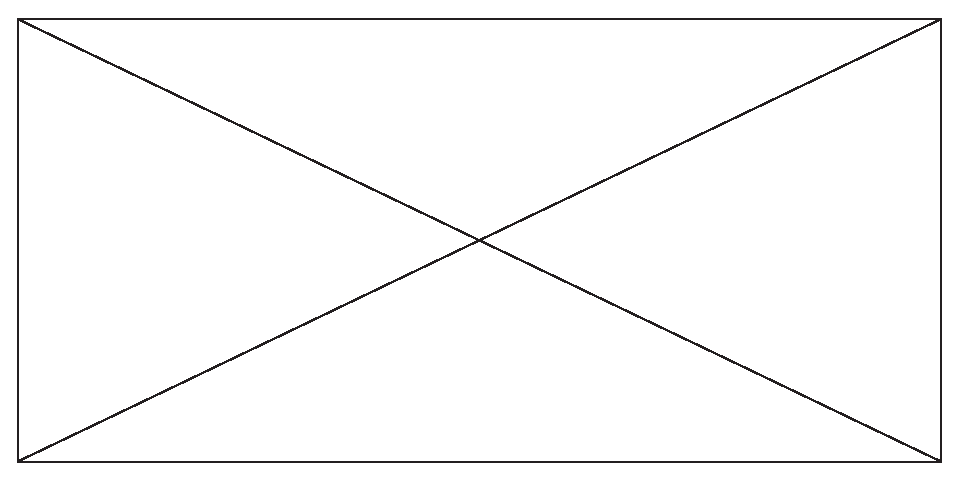
\includegraphics[width=\textwidth, height=\measurepage]{img/fill_page.eps} \newpage}

\newenvironment{itemize*}%
{\begin{itemize}%
		\setlength{\itemsep}{1pt}%
		\setlength{\parskip}{1pt}}%
	{\end{itemize}}


\newenvironment{enumerate*}%
{\begin{enumerate} %
		\setlength{\itemsep}{1pt}%
		\setlength{\parskip}{1pt}}%
	{\end{enumerate}}

%\newcounter{number_of_meeting}\setcounter{number_of_meeting}{0}

\renewcommand{\labelenumii}{\arabic{enumi}.\arabic{enumii}.}
\renewcommand{\labelenumiii}{\arabic{enumi}.\arabic{enumii}.\arabic{enumiii}.}
\renewcommand{\labelenumiv}{\arabic{enumi}.\arabic{enumii}.\arabic{enumiii}.\arabic{enumiv}.}
\pagestyle{fancy}
{
\fancyhead{}
\fancyhead[C]{PML30 Saint-Petersburg}
\fancyfoot{}
\fancyfoot[LE,RO]{\thepage}
\fancyfoot[C]{Russia, St. Petersburg, Physics-Mathematics Lyceum №30. 2014-2015}
}


\begin{document}

	
	%\thispagestyle{titlestyle}
\begin{titlepage}
	
	\begin{center}
		\LARGE\textit{Center for robotics \\ Physics-Mathematics Lyceum 30}
        \begin{figure}[H]
         	\center{
	            
\includegraphics[scale=0.45]{days/Title/images/01}  
				
\includegraphics[scale=0.15]{days/Title/images/02}
			}
        \end{figure}
		\vspace{3em}
		
		\LARGE{Engineering book of \\ Competition First FTC}
		
		\vspace{2em}
		
		\bf\fontsize{50}{60}\selectfont Team PML30-${\varphi}$ \\ 9746 \fontsize{11}{13}\selectfont
			
	\vspace{6em}
		
		\begin{figure}[H]
			\center{
			    
\includegraphics[scale=0.12]{days/Title/images/03}  
		        
\includegraphics[scale=0.7]{days/Title/images/04}
		        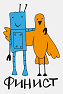
\includegraphics[scale=1.1]{days/Title/images/05}
		        
\includegraphics[scale=0.3]{days/Title/images/06}
			}
		\end{figure}
			
		\LARGE\normalfont Saint-Petersburg, Russia	\\ 2015
	\end{center}
\end{titlepage}

\newpage

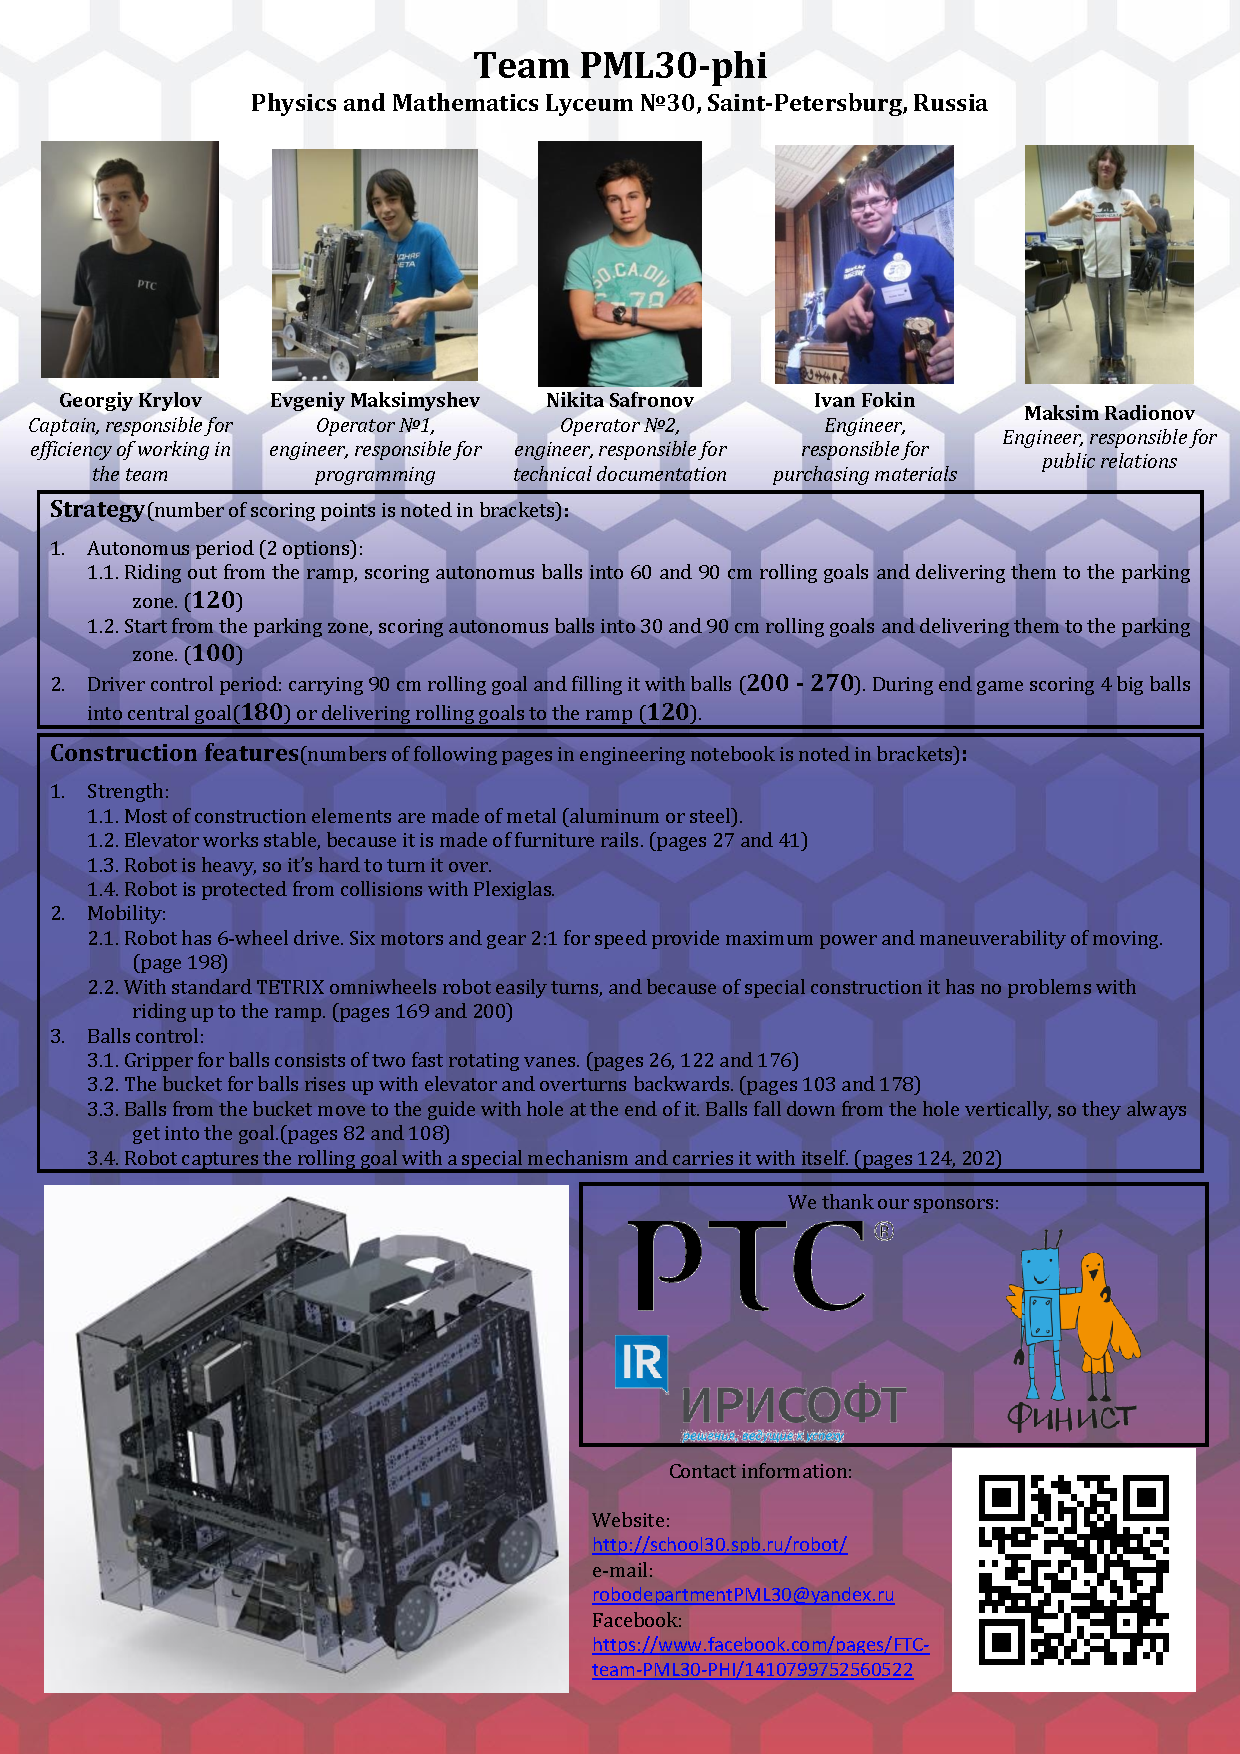
\includegraphics[scale=0.8]{days/Title/images/PML30-PHI-infolist_judge}


	
	%\tableofcontents{}
	%\newpage
	
	\chapter{How to read this book}
	\subsection{Introduction}
	
	
	\subsection{Structure of the book}
		
		
	\subsection{Navigation}
	
	
	\subsection{Thesaurus of specific words}
\newpage	
	%
\section{Team PML 30 X} 
	Team PML 30 X was assembled in September 2014 in the Russian city of St. Petersburg from 3 novices and 2 participants with experience. Tasks and roles were distributed among the participants, and we established safety rules. In the first place the team put spreading principles of gracious professionalism to others. All decisions were made collectively inside team with discussion to find the most optimal solutions. 
	During the year we took part in many events and everywhere we have tried to attract attention to our team and encourage people to take part in FTC. Also we pursued and distributed the principles of honorable professionalism. Talking to the press, we hoped to attract more attention to our team and to the competition in general, as well as attracting sponsors. The latter was important because of the need for funds - purchasing materials and equipment costs a lot.
	Last season the team took part in the three qualifying competitions, in the regional finals, in European championship and in the World championship. In all of them we made new contacts, shared experience and provided mutual assistance to other teams. In the first qualifying rounds in Sochi we met Stuy Fission 310 from USA and maintain contact with them to this day. On regional finals, we met with a team from Romania, Auto Vortex, and keep in touch with them through Facebook. Also, there is an active group chat with a large number of Russian teams. You can find the team page in Facebook at the address https://www.facebook.com/pages/FTC-team-PML30-X.
	To increase the efficiency of our team work we used the version control system GitHub, which allows the entire team to work simultaneously on a single projects without losing files and providing easy way to resolve roblems. Also for writing technical books we been used professional typesetting system LaTeX.
	\begin{figure}[H]
		\center{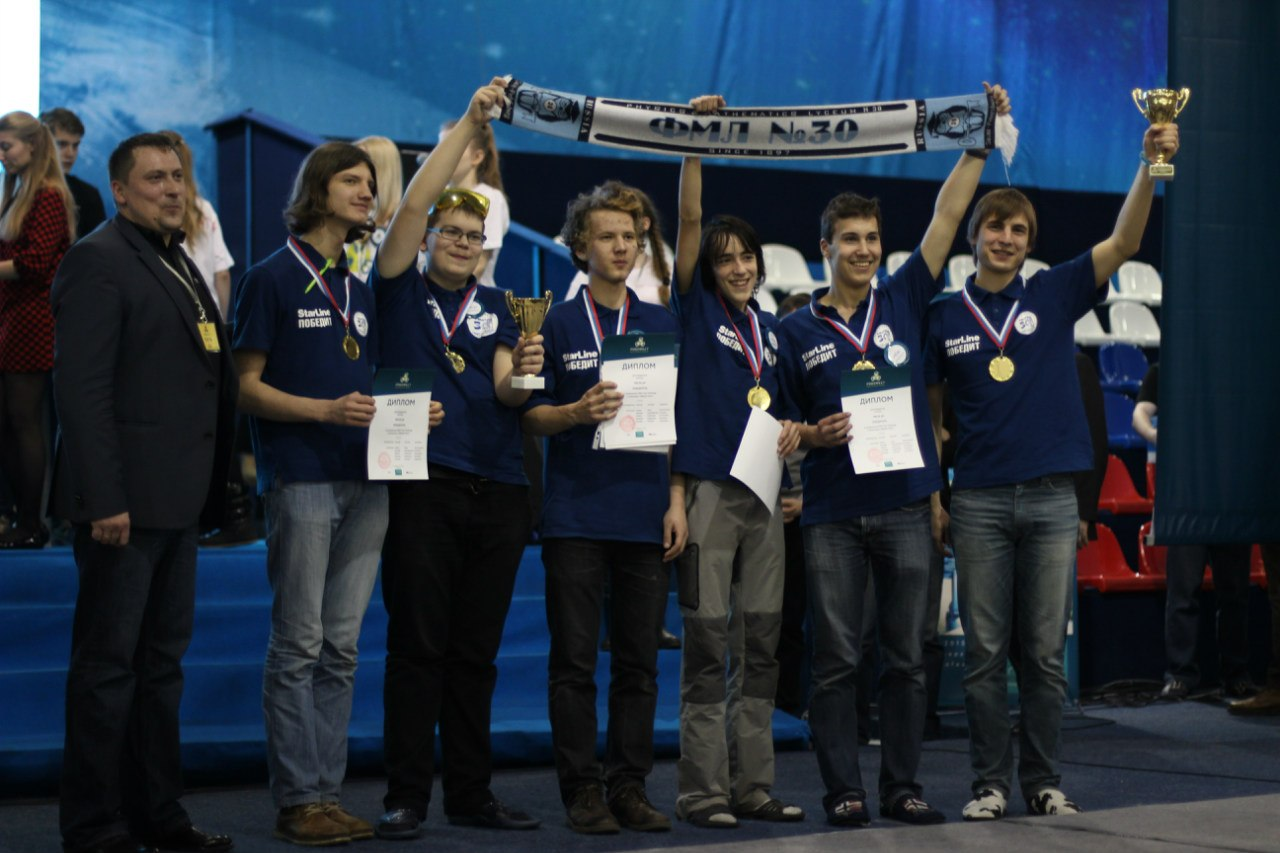
\includegraphics[scale=0.2]{key_chapters/Team/images/09}}\\
	\end{figure}[H]
\fillpage

\subsubsection{Instructors}:

\begin{figure}[H]
	
	\begin{minipage}[h]{0.47\linewidth}
		Luzin Dmitry\\
		\emph{Head of Robotics Department in Phys-Math Lyceum 30, Saint-Peterburg, Russia. Main coach of FTC team.\\}
		\emph{Information: 26 years old, in robotics 6 years, in FTC 4 years.}
	\end{minipage}
	\hfill
	\begin{minipage}{0.47\linewidth}
		\center{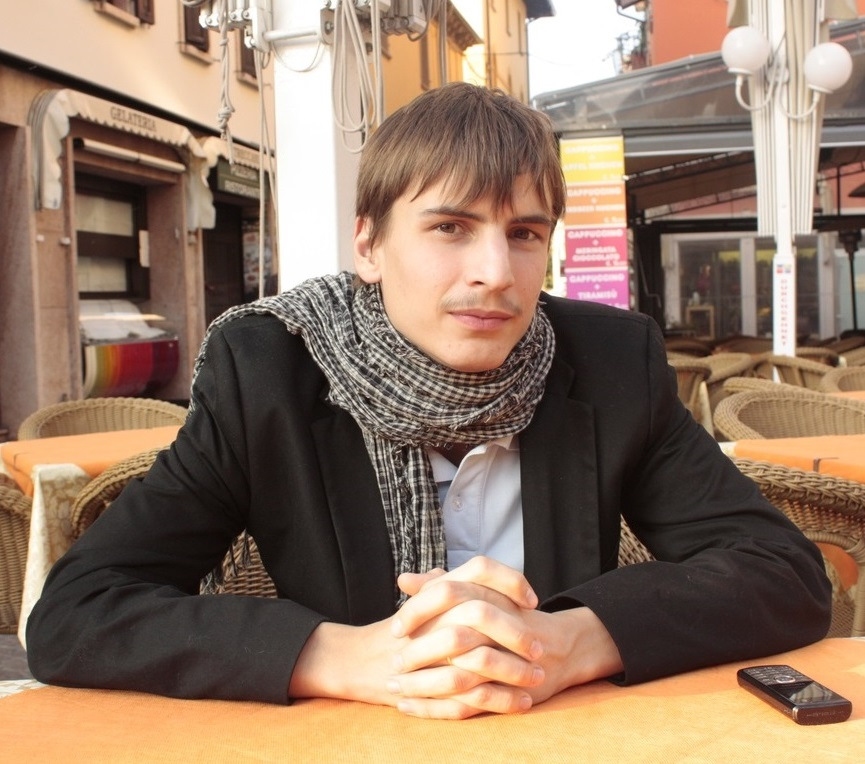
\includegraphics[scale=0.3]{key_chapters/Team/images/07}}\\
	\end{minipage}
	\vfill
	\begin{minipage}[h]{0.47\linewidth}
		\center{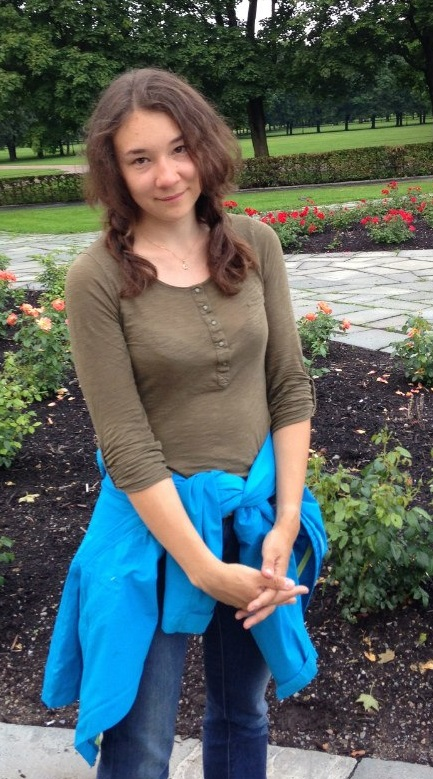
\includegraphics[scale=0.35]{key_chapters/Team/images/08}}\\
	\end{minipage}
	\hfill
	\begin{minipage}{0.47\linewidth}
		Luzina Ekaterina \\
		\emph{Professor of Robotics Department in Phys-Math Lyceum 30, Saint-Peterburg, Russia. Tutor of FTC team. \\}
		\emph{Information: 26 years old, in robotics 6 years, in FTC 4 years.}
	\end{minipage}
\end{figure}

\begin{figure}[H]
	\begin{minipage}[h]{0.47\linewidth}
		\center{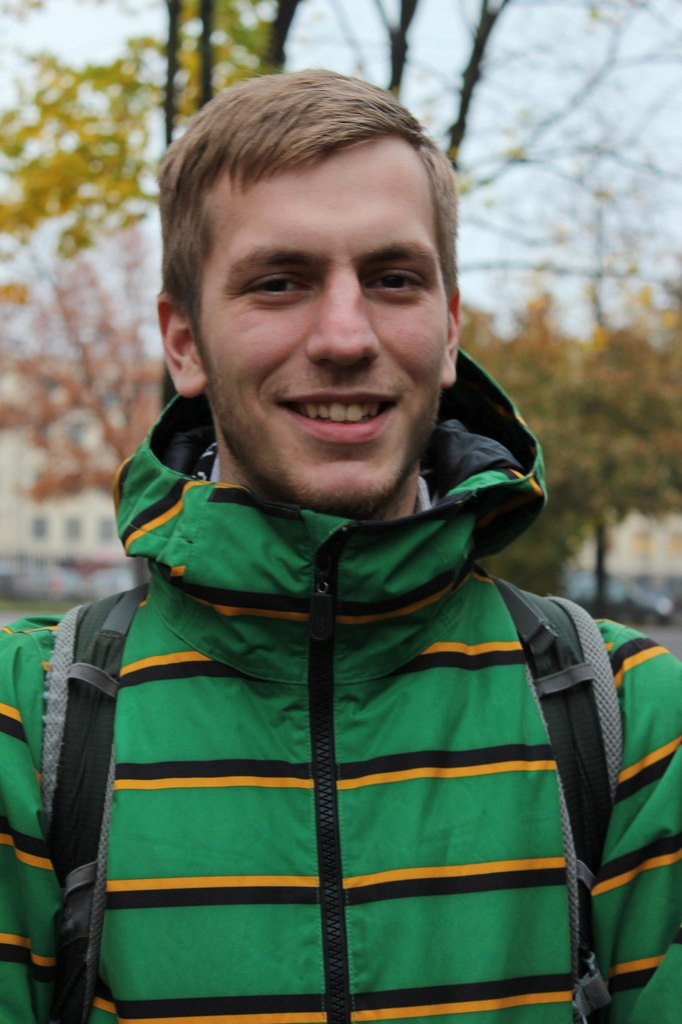
\includegraphics[scale=0.25]{key_chapters/Team/images/05}}\\
	\end{minipage}
	\hfill
	\begin{minipage}{0.47\linewidth}
		Fedotov Anton \\ 
		\emph{Professor of Robotics Department in Phys-Math Lyceum 30, Saint-Peterburg, Russia. Tutor of FTC team. \\}
		\emph{Information: 23 years old, in robotics 5 years, in FTC 4 years.}
	\end{minipage}	
	\vfill 
	\begin{minipage}[h]{0.47\linewidth}
		\center{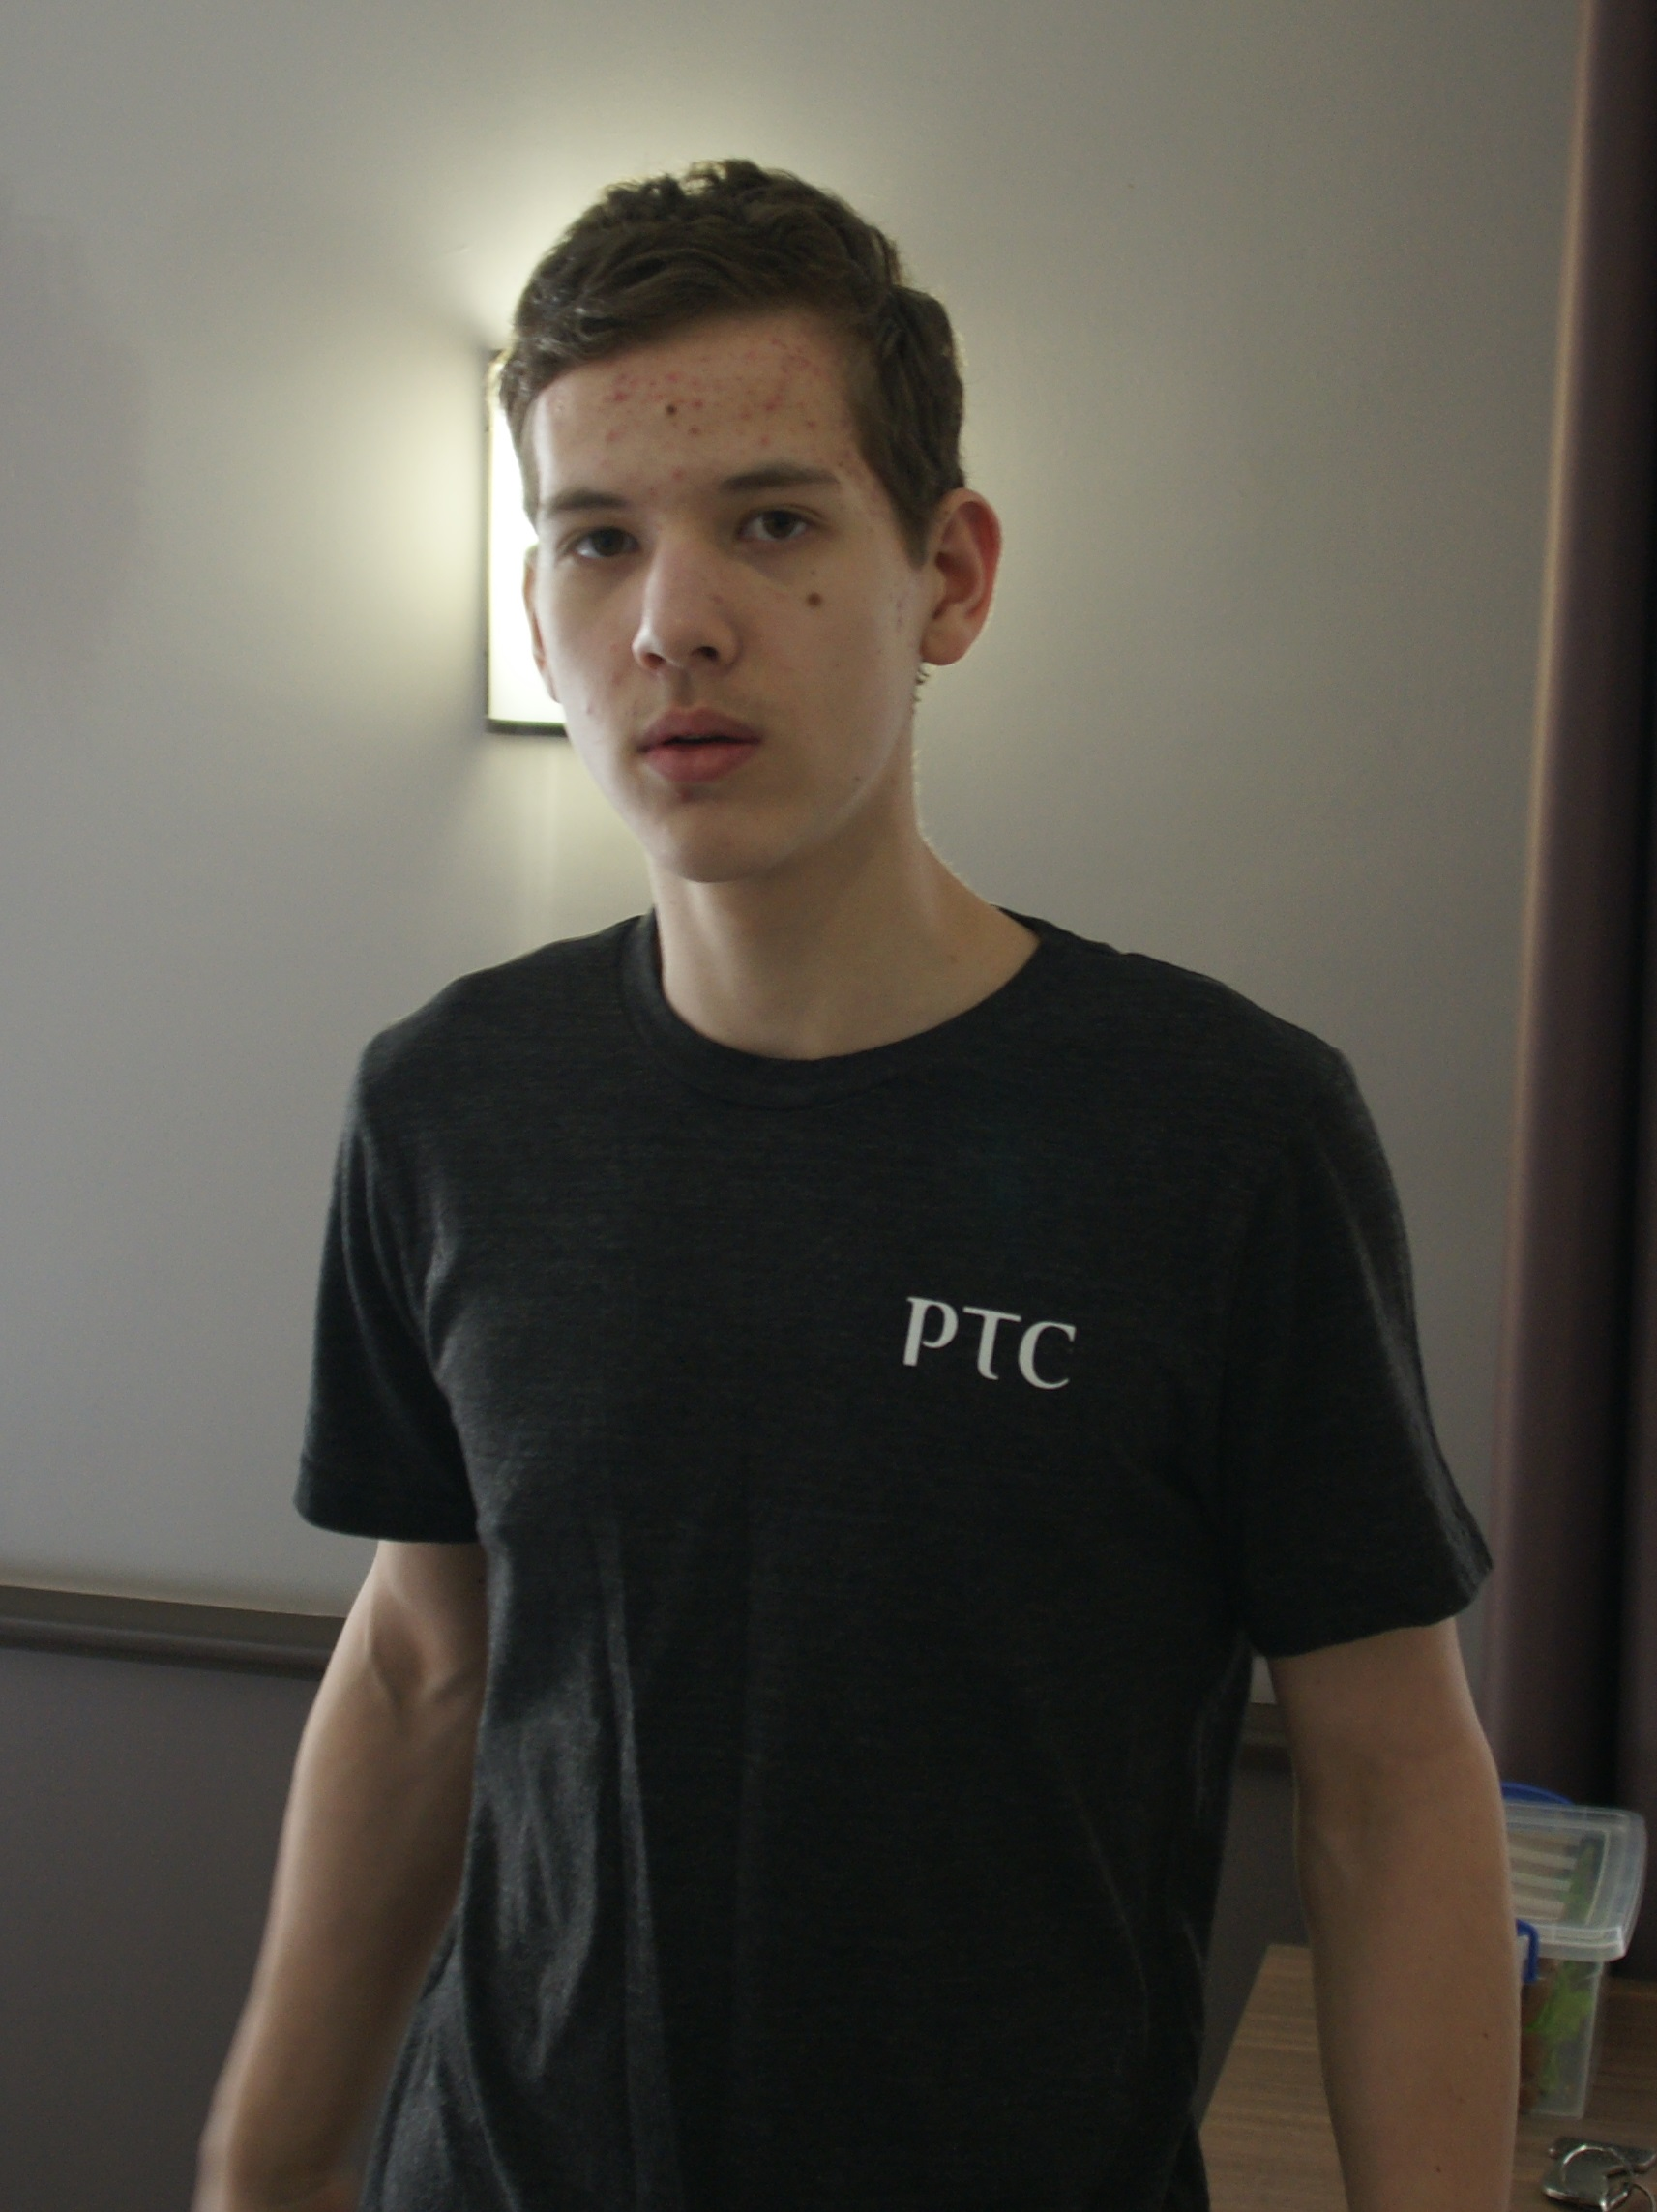
\includegraphics[scale=0.1]{key_chapters/Team/images/06}}\\
	\end{minipage}
	\hfill
	\begin{minipage}{0.47\linewidth}
		Krylov Georgii \\ 
		\emph{Professor of Robotics Department in Phys-Math Lyceum 30, Saint-Peterburg, Russia. Tutor of FTC team. \\}
		\emph{Information: 18 years old, in robotics 4 years, in FTC 4 years.}
	\end{minipage}	
\end{figure}

\fillpage

\subsubsection{Team members}
\begin{figure}[H]
	\begin{minipage}[h]{0.47\linewidth}
		\center{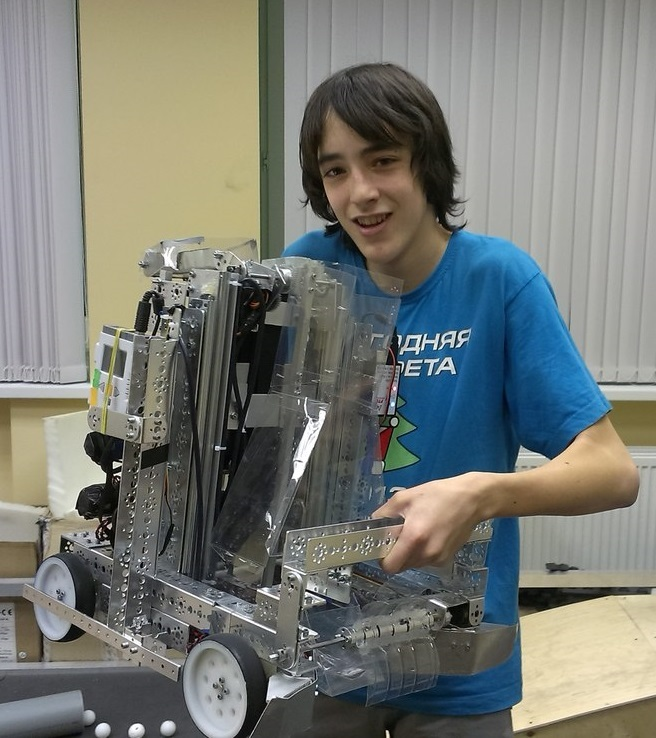
\includegraphics[scale=0.27]{key_chapters/Team/images/04}}\\		
	\end{minipage}
	\hfill
	\begin{minipage}[h]{0.47\linewidth}
		Maksimychev Evgeny\\
		\emph{Role in team: captain, operator-2, responsible for the technic of safety,  writing of engineering notebook, developer of lift and bucket for scoring elements. \\}
		\emph{Information: 16 years old, in robotics 3 years, in FTC 2 year. \\}
		\emph{Why I chose FTC: "This is an interesting project that allows to implement some innovative solutions. In addition to the skills of designing robots, we also obtain the skills of the technical documentation and communication with colleagues which makes this competition as close to real engineering problems."}	
	\end{minipage}
\end{figure}
	\vfill 
	\begin{figure}[H]
	\begin{minipage}[h]{0.47\linewidth}
		Timur Babadzhanov\\
		\emph{Role in team: operator-1,  developer mechanism for scoring autonomous climbers\\ }
		\emph{Information: 15 years old, in robotics 2 years, in FTC 1 years. \\ } 
		\emph{Why I chose FTC:" It was recommended for me. Also I heared about previous seasons of FTC and decided that it will be interesting for me. Also I wanted to learn working with TETRIX that can be useful for my projects."}					
	\end{minipage}
	\hfill
	\begin{minipage}[h]{0.47\linewidth}
		\center{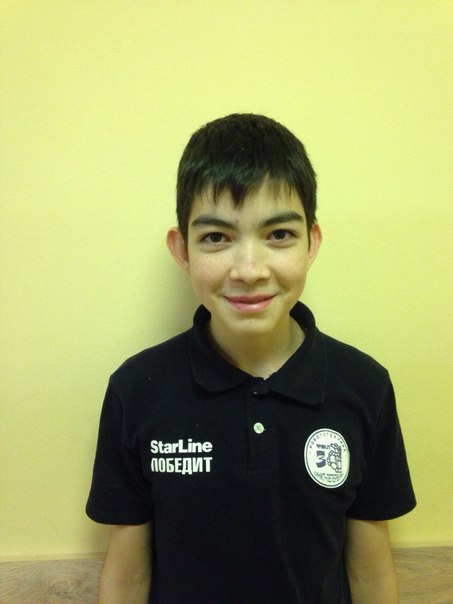
\includegraphics[scale=0.4]{key_chapters/Team/images/01}}\\
	\end{minipage}
\end{figure}
\hfill

\begin{figure}[H]	
	\begin{minipage}{0.47\linewidth}
		\center{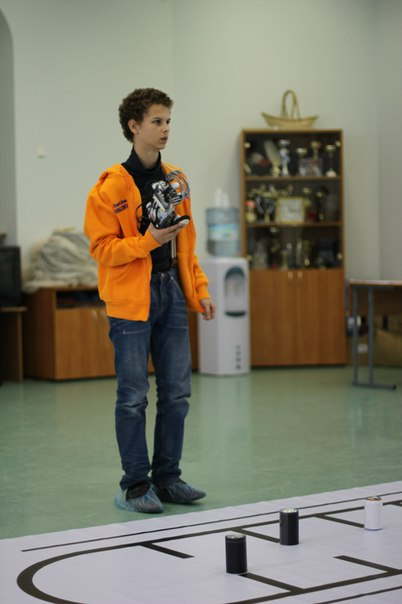
\includegraphics[scale=0.6]{key_chapters/Team/images/10}}			
	\end{minipage}
	\hfill
	\begin{minipage}{0.47\linewidth}
		Ivan Afanasev\\
		\emph{Role in team: developer of gripper for debris\\ }
		\emph{Information: 16 years old, in robotics 2 years, in FTC 1 years. \\ } 
		\emph{Why I chose FTC:" It is a good realization of my engineering skills. I'm good at physics and programming and decided try robotics as merger of this subjects. FTC give opportunity to learn, meet with people from other contries. It is good for pupils such as I."}		
	\end{minipage}
\end{figure}
\hfill
\begin{figure}[H]	
	\begin{minipage}{0.47\linewidth}
		Victoria Loseva\\
		\emph{Role in team: developer of wheel base\\ }
		\emph{Information: 17 years old, in robotics 2 years, in FTC 1 years. \\} 
		\emph{Why I chose FTC:"I enjoy working on new and unique projects, and FTC is a great way for me to do exactly that: solving the challenging problem of building and designing a robot from scratch, as a team, is all it's about!"}			
	\end{minipage}	
	\hfill
	\begin{minipage}{0.47\linewidth}
		\center{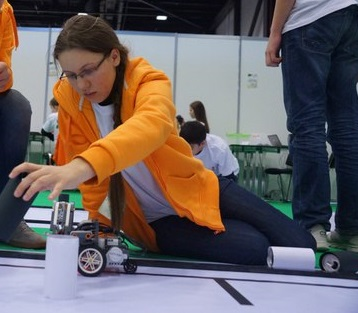
\includegraphics[scale=0.7]{key_chapters/Team/images/11}}			
	\end{minipage}
\end{figure}
\fillpage



	%\section{Events}
	\subsubsection{Qualifying competitions}
		\begin{enumerate}
			\item Sochi. 21-23.11.2014. 
			Sochi was the first time the team participated in a comptetition. There, our team felt the spirit of FTC comptetion and noble professionalism for the first time. We got work experience all day and all night, began to make acquaintance among the teams, and providing all possible help we could. The planning and organization were all very nice. The most memorable contact we made was with the American team Stuy Fission 310, with which we now keep in touch. As a result we won a Think Award and a pass to the Regional final.
			\begin{figure}[H]
				\center{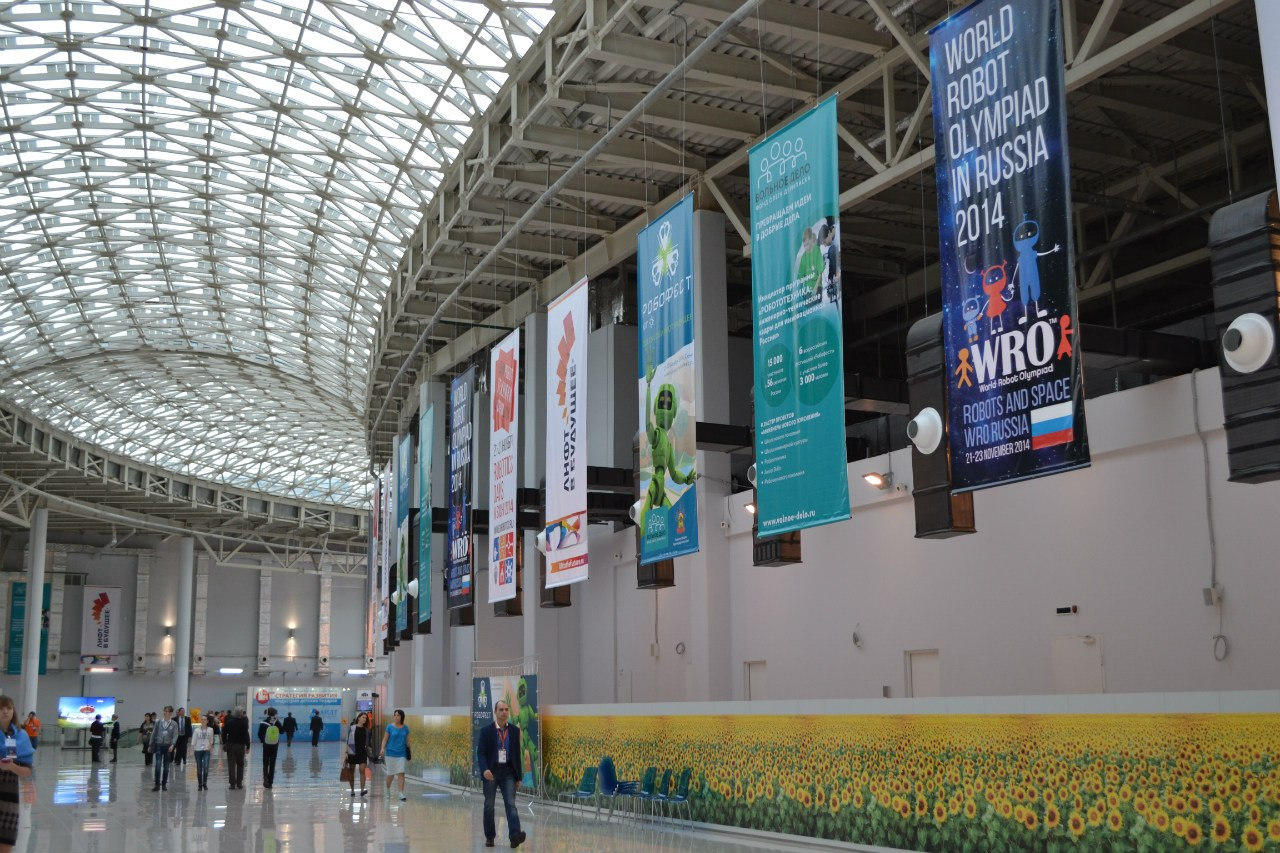
\includegraphics[scale=0.25]{days/Events/images/6}}
			\end{figure}
			\item Ryazan. 13-14.12.2014. 
			Our first priority was to train on a real field. These competitions were quite small and quiet, all the teams communicated abundantly and shared ideas freely. We all felt comfortable there. The team helped to assemble and disassemble the field. As a result - Winner Alliance Award and Think Award. 
			\begin{figure}[H]
				\center{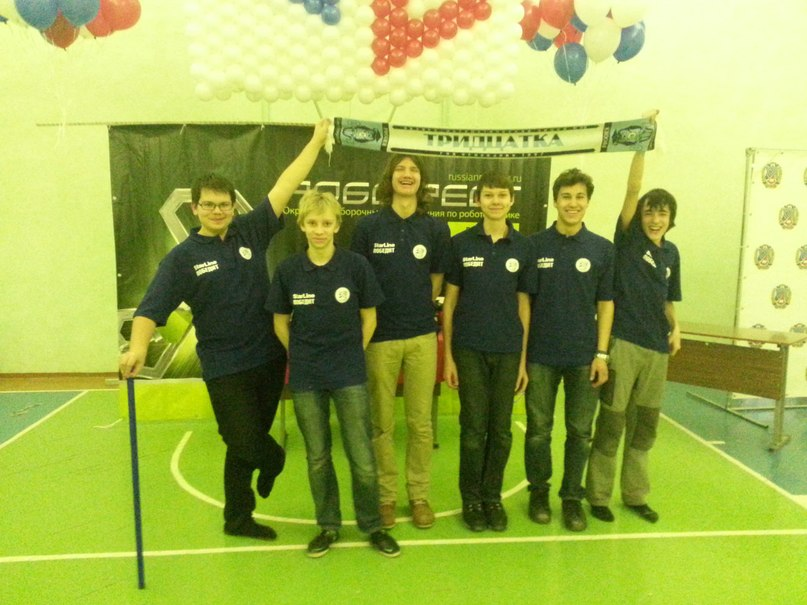
\includegraphics[scale=0.4]{days/Events/images/1}}
	     	\end{figure}	
			\item Perm. 27-29.01.2015. 
			Dress rehearsal before the regional final. It was great organized event where we were able to practice all aspects of the competition. Including such important skills as the choice of Composes alliances finale. Also we strongly helped to organized technical part. As a result - the Winner Alliance Award and Inspire Award.
			\begin{figure}[H]
				\center{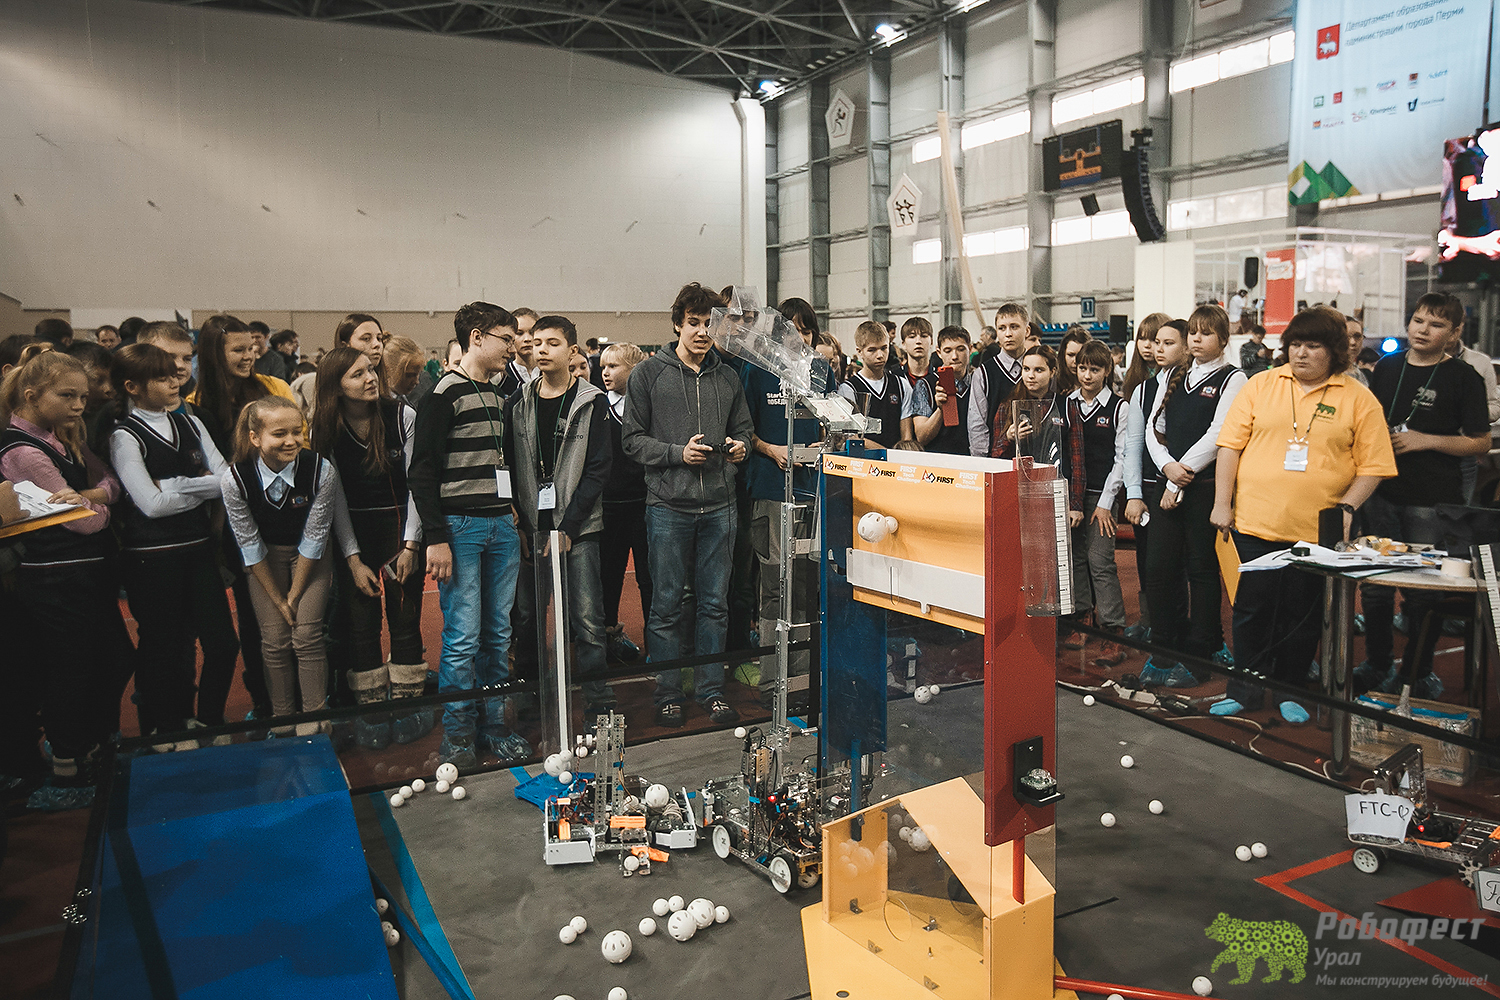
\includegraphics[scale=0.22]{days/Events/images/3}}\\
	     	\end{figure}
		\end{enumerate}  
	\subsubsection{Regional final. 11-13.02.2015}	
	This was the event, to which the team had been preparing for for six months. Approaching the competition with fully finished. At competitions communicated with all the teams that were there, discussing strategy and offering their help. During the competition statistics were conducted on all the teams. It helped in choosing allies for the final. Was also had an action plan for an alliance with any team. In the final, having received a the choice of allies, we chose the team with the most stable results, and the bet was at collaborative interaction of any pair of robots. Results: Winner Alliance Award, Inspire Award and the pass to World Championship in Saint Louis.
	\begin{figure}[H]
		\center{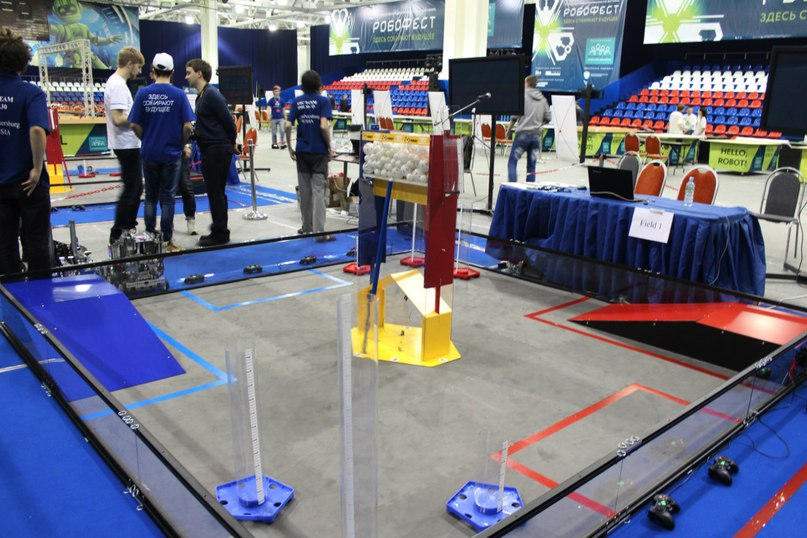
\includegraphics[scale=0.45]{days/Events/images/2}}\\
	\end{figure}
	\newpage			
	\subsubsection{CRDI RTC. 24.11.2014}
	Central Russian Institute of Robotics and Technical Cybernetics. A tour was organized for the team in the institute, where we could see the real processes of development of detailed design for robotics. There we saw several project summaries at different stages of development - from drawings to finished models, as well as commercially ready products. From there we learned some ways on how to organize. Internet adress http://www.rtc.ru.
	\begin{figure}[H]	
		\center{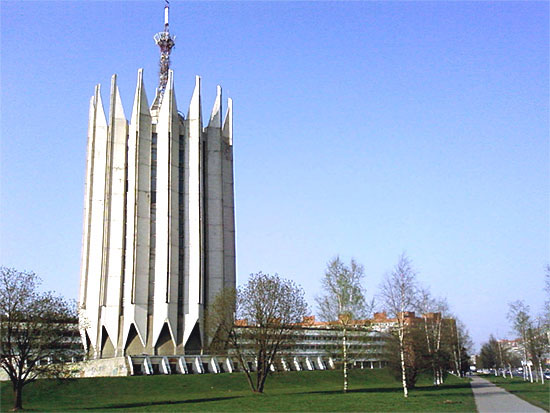
\includegraphics[scale=0.5]{days/Events/images/5}}\\
	\end{figure}
	\subsubsection{PML30 POLYGON. 08.02.2015}	
	PML30 POLYGON competitions are carried out by our organization. Their main  misrepresented that participant receives a rear and parts for its decision merely on the competition, compliance with the maximum being equal. We also demonstrated the FTC involving the participation.
	\begin{figure}[H]
		\center{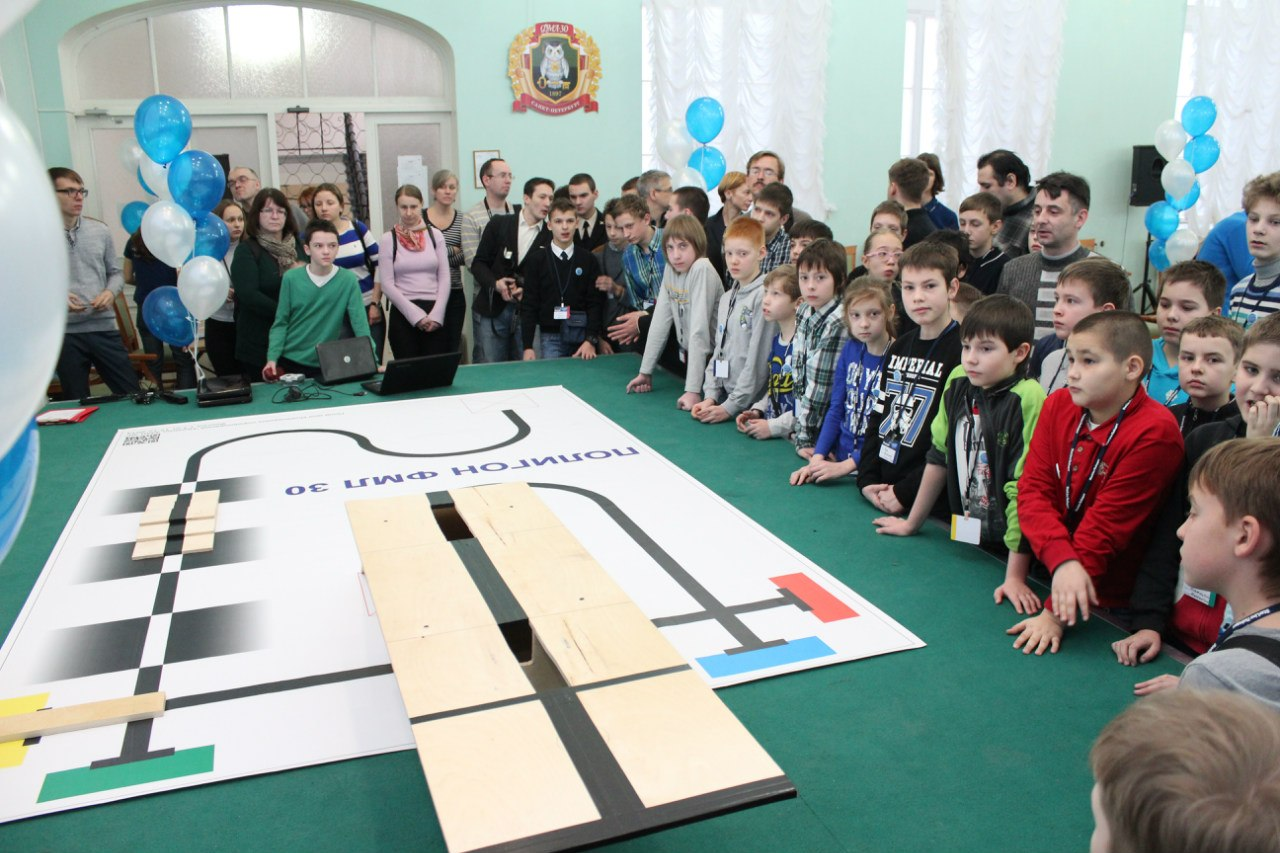
\includegraphics[scale=0.25]{days/Events/images/7}}\\
    \end{figure}
    \subsubsection{GeoScan. 10.03.2015}
	A Russian company thatproduces and sells unmanned aerial photography systems. There we were clearly shown how the office is designed, as well as the distribution of responsibilities and tasks, and what the internal interaction is like. Also, we were shown the whole production line. Internet adress http://geoscan.aero/.
    \begin{figure}[H]
    	\center{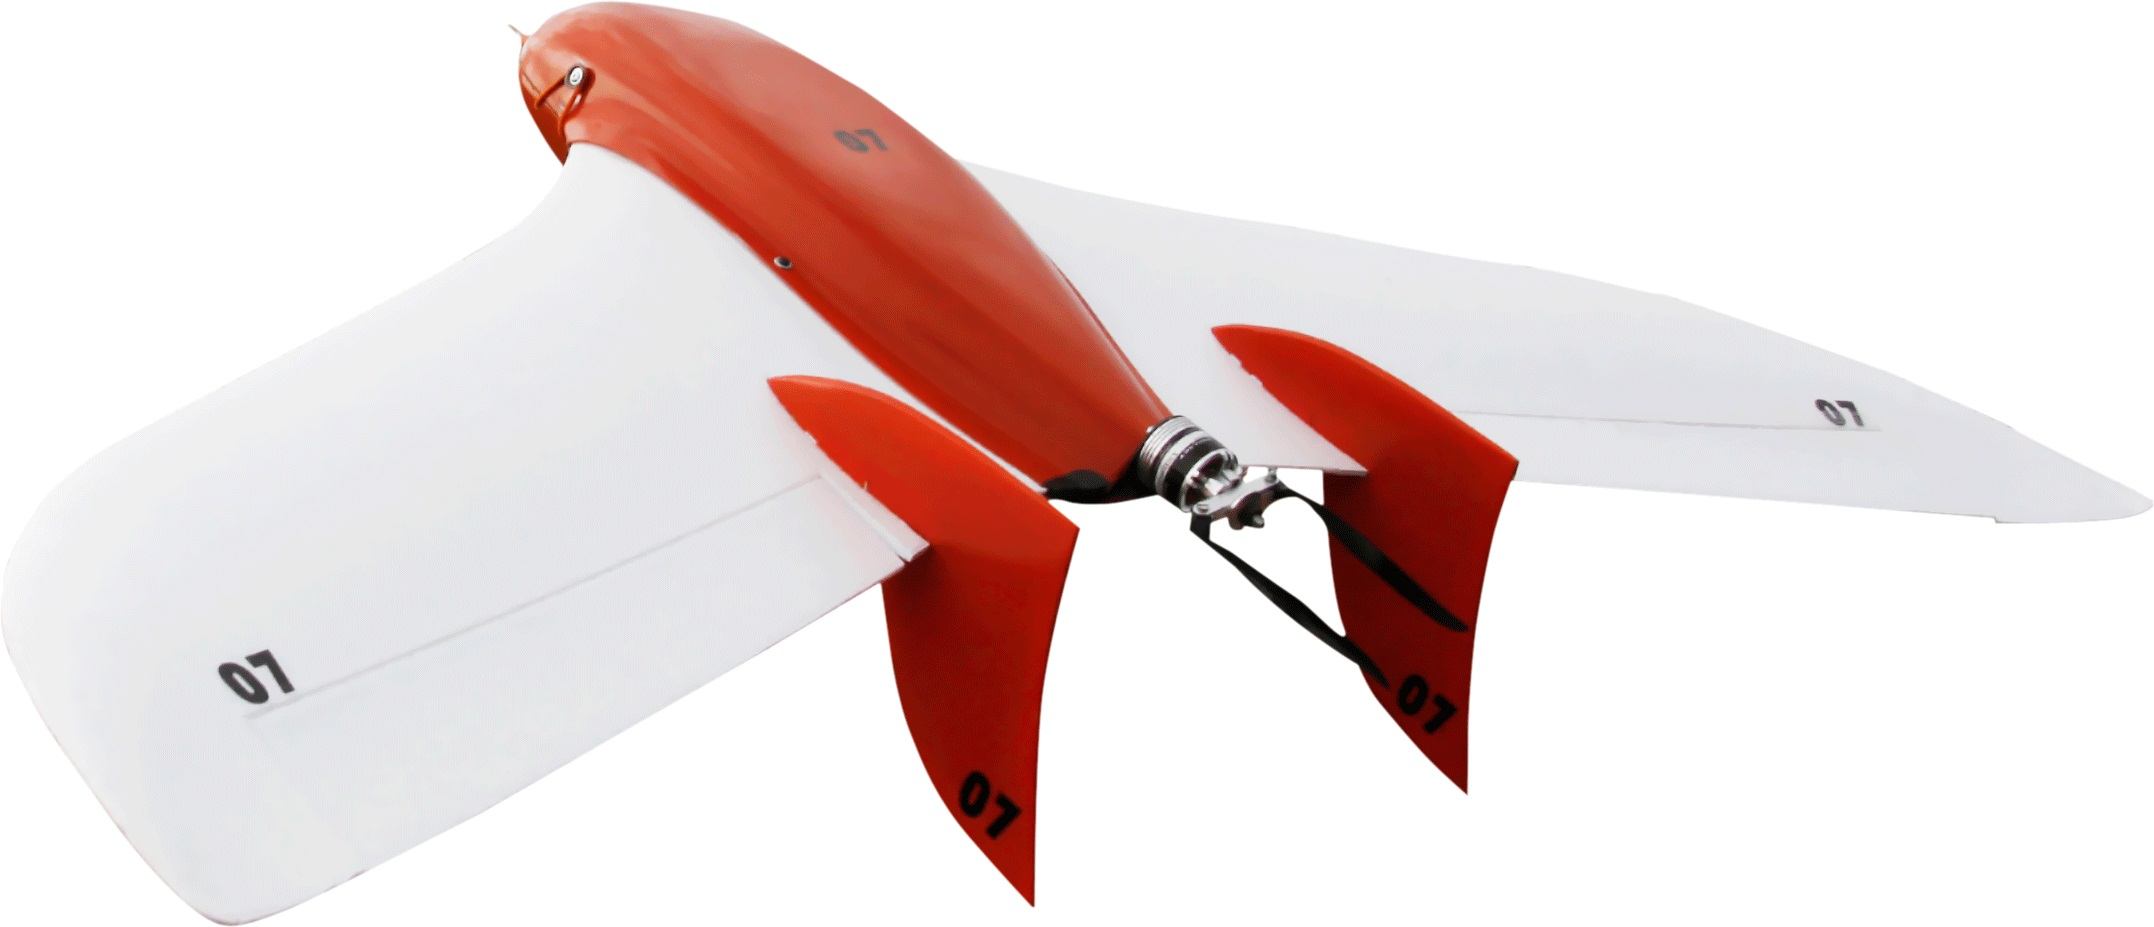
\includegraphics[scale=0.2]{days/Events/images/4}}\\	
    \end{figure}
	\subsubsection{PTC live Tech Forum. 24.03.2015}
	 The team was invited to participate in PTC Live Tech Forum. We will present the successfull path of 3D model creation in Creo Parametric, tell about important tips and show how CAD modelling helped us to build the robot.
	
	\subsubsection{Summer camp on Robotics}
	In the camp in 2015, team members will conduct a robotics engineering course based on constructor TETRIX, attracting more people to the FTC.
	
	\fillpage
		
		
		
		
		
		
		
		
		
	%\section{Business plan}
	\subsection{introduction}
	We take a responsible approach to finding sponsors. And also try to spend money effectively advance thinking through the details and equipment, finding ways to get them maximum benefit. Some sets we received as prizes in competitions.
	
	\subsection{Our sponsors and their support}
		\subsubsection{PTC and Irisoft}
		PTC and Irisoft representative in Russia is the one company that has helped us to begin to engage FTC. They provided us the first set of Tetrx within the program's Score Thehnic which involved our Lyceum. They provide us with a different command symbols plus small gifts for other teams. They help us with the delivery of details from U.S.A. We use them programa Creo for creating 3D models. We also take part in events organized by them.
		\subsubsection{Robofinist}	
		Robofinist Charitable Foundation organized by Temur Amindzhanov and by Starline. They offered us its assistance as an organization in our city with outstanding achievements. They help to financially each month to give us 2000 Dolars, parts and equipment.
		\subsubsection{Volnoe Delo}
		Volnoe Delo is one of the largest charitable foundations in Russia. It was established by Oleg Deripaska. We are participants of the program ROBOTOTEHNIKA.As support they sent us free game field.They also engaged in training teachers and judges, including our own.They engaged in the organization of competitions FTC in Russia and are sponsoring a trip this year's winners to St. Louis.	
		\subsubsection{Physics-Mathematics Lyceum №30}
		Physics-Mathematics Lyceum №30 is a school in which is our organization. It provides us with a comfortable space and material assistance, as well as leaders.
		
	\subsection{Purchase of materials.}
		\subsubsection{Our method}
		When we started robotics we had not a lot of money and we used only some basic materials. Now we found sponsors and firstly plan the details and equipment that we need to buy and then buy them.Such an approach allows us to find more effective solutions.
		\subsubsection{Our materials}
		We have 6 primary kits and 3 resource kits.We buy individual parts we need.At this point was made 2 large purchases from U.S.A for 1600 Dolar in November 2014 and March 2015.
\newpage	
	
	\subsection{Brainstorming (21.09.2015)}
	\textit{\textbf{Time frame:}} 21.09.2015 17:00-21:00 \newline
	\textit{\textbf{Preview:}} Since this year FTC rules were published, every member of our team had carefully read them. Today we gathered together to discuss all the aspects of this year gameplay and think of how to get on with the most significant features of the game. \newline \newline
	\textit{\textbf{General aspects:}}
	\begin{table}[H]
		\vspace{-2mm}
		\begin{center}
			\begin{tabular}{|p{0.4\linewidth}|p{0.5\linewidth}|p{0.1\linewidth}|}
				\hline
				Features & Solutions & Label \\
				\hline
				Moving to the ramp is essential to achieve high score. & Robot's wheel base should be good at moving on the ramp. & chassis \\
				\hline
				Space between each two bars in 3-rd zone is wider than the standard TETRIX wheel diameter. & Using tracks or 3-4 wheels from each side of the robot will prevent robot from getting stuck. & chassis \\
				\hline
				It will take a lot of time to climb to the 3-rd zone of the ramp. & It is possible to deliver debris to the highest goal with elevator standing on the 2-nd zone instead of climbing to the 3-rd. & elevator \\
				\hline
				Goals for debris have a very little capacity. & It is more preferable to collect cubes than balls. That's why we need mechanism to prevent balls from collecting. & gripper \\
				\hline
				Pulling up costs 80 points. It's not difficult to realise then. & At least 1 DC motor should be reserved for pulling up. It is possible to grasp the pull-up bar with hook and lift to it by reeling the cable. & pull up \\
				\hline
				Moving over the inclined plane and pulling up require high moment on motors. However, the number of motors is limited. & Robot should be light enough to decrease the moment required for moiving and, as a result, increase speed of moving. & weight \\
				\hline
				All the zones of red alliance are the mirror reflection of blue alliance's zones. & Robot should be symmetrical and capable of playing on both sides of field. & concept \\
				\hline
				Robot can grip 5 debris at once, when the maximal capacity of one bucket is 24 cubes. So, to fill one bucket robot has to repeat collecting and taking cubes to the goal 5 times per 1,5 minutes & Gripper for debris should be at the front side of the robot and extractor for scoring elements - from the back side. It will allow robot to go to the ramp backwards, so it won't need to turn around on the ramp before going down to collect debris. It will save some time. & concept \\
				\hline
				It's quite unconvenient to exchange ramps with your ally during the game. & We will negotiate with our ally about spheres of influence before each game. Additionally, there should be two autonomus programs for climbing onto both ramps. & strategy \\
				\hline
				The only main difficulty of this year autonomus period is that both robots in alliance have to fulfil the same tasks at the same place. So, there is a high risk of collisions between them. & A number of different programs for autonomus period are needed for easier adjustment to the ally's strategy. & strategy \\
				\hline
				It's not restricted to collect debris in autonomus period. & It will be useful to realise automatic collection of 5 cubes in autonomus period. At the conclusion of autonomus period the robot will remain on the ramp with 5 cubes and we will put them to the goal immediately & strategy \\
				\hline
			\end{tabular}
		\end{center}
	\end{table}
	
	 \newline
	\textit{\textbf{Detailed explaination:}}
	\begin{enumerate*}
		\item As we know from our previous FTC seasons experience, there are strict constraints for wheel bases can be used for climbing mountains. Firstly, omni and mechanium wheels are completely not suitable, because mechanium wheels can ride only on plain surface (when 2-nd and 3-rd zones have cross hurdles) and omni wheels have ability of undependable movement on small rollers so they behave very unstable on mountain. Various conbinations of standard and omni wheels can't be used too, as in the 2-nd zone there are obstacles which can cause some wheels lose contact with ground and if the rest of wheels will behave differently, the whole robot would be unstable. In conclusion, we can use only standard wheels or tracks.
		
		Additionally, wheel base should be symmetrical against central axis for stable climbing to the mountain.
		
		If we decided to climb 3-rd zone with standard wheels, we will have to put 3-4 wheels at the each side to avoid getting stuck on hurdles (the space between two hurdles is for about 14 cm, when the diameter of big TETRIX wheels is only 10 cm).
		\begin{figure}[H]
			\begin{minipage}[h]{1\linewidth}
				\center{
\includegraphics[scale=0.2]{00.00.2015/images/01}}
				\caption{possible wheel bases}
			\end{minipage}
		\end{figure}
		% % % %
		\item To score in high zone goal from 2-nd zone robot should have a mehanism for delivering debris to the distance of 40 cm or more. Shooting debris is entirely unsuitable approach, because it's impossible to realise enough accuracy for stable scoring cubes and especially balls. Another way is elevator. There are three types of lifts which familiar to us: they're crank lift, scissor lift and retractable rails. 
		
		Scissor lift is not suitable for this year competition, because despite it's main advantage - the ability of extracting the longest distances of all - it's too difficult in development.
		
		Crank lift allows to vary the angle of turning of each segment. However, it requires at least one DC motor of strong servo for every joint.
		
		Retractable rails can only move along one axis. However, they require the least space and can be equipped by one DC motor (as all the motors are connected to the only reel, which winds the cable).
		\begin{figure}[H]
			\begin{minipage}[h]{1\linewidth}
				\center{
\includegraphics[scale=0.2]{00.00.2015/images/02}}
				\caption{types of elevators}
			\end{minipage}
		\end{figure}
		% % % %
		\item The parameters of the box are $9\times5.75\times6.25$. So, it can contain at most 24 cubes (4 in length, 2 at width and 3 in depth). As for balls, there can't be scored over approximately 10 of them because of their unconvenient shape and ability of top balls to roll out of the box (especially from the upper box, which is turned on $50^{\circ}$ from horisontal position).
		
		This is the reason to implement mechanism for separating debris into cubes and balls. However, there are only 50 cubes on field (12.5 for one robot), so they will run out quickly, so the ability of collecting balls is required as well.
		
		Additionally, we need to think of how to put cubes into boxes gently so as they will settle down in straight lines. It will allow entire filling boxes with cubes.\newline
		% % % %
		\item Solid constructions for pulling up will be too bulky because they have to be strong enough to withstand full weight of the robot. The more reliable and simple solution is steel cable with hook for grasping the bar on it's tail.
		
		In second case the most difficult objective is to deliver hook to the bar, which can be solved by creating secondary lift for it (the main one is a lift for debris). Mechanism for shooting hook towards the bar is not suitable as it can be dangerous for operators and spectators (if the it will be accidentally activated during the match).\newline
		% % % %
		\item The main weight of the robot goes the battery and motors. The weight of the battery is 570g. We have two types of motors: standard TETRIX motor (207g) and "NeveRest 40" motor by AndyMark (334g). The complete control system (phone + controllers + power distributor) weigh about 700g.
		
		Therefore, total weight of essential components varies from 2926g to 3942g (with 8 motors). With several beams (166g the longest), wheels (117g each) and other construction elements robot will weigh from 6 to 10kg. 
		
		In our primary calculations robot's weight will be accepted as 10kg. However, it is preferable to make robot as light as possible.\newline
		% % % %
		\item Wheel bases which are good at climbing mountains are usually less manevrous, than carriages with omni and mechanium wheels. This way, the less robot will turn, the more effective it will compete.
		
		Accordind to this, it will be more convenient to realise construction that will allow robot to score debris without turning around. Robot can collect debris with gripper on it's front side while moving forward and then go backward to the ramp and score debris with the mechanism on it's back side.
		
		Furthermore, it will be useful to attach one robot to one ramp in order to prevent them from commiting extra movement. Although it seems that two robots can fill the top goal together two times faster, in fact they will just interfere with each other. So, it will be a good tactical step to negotiate with our ally before the mach which robot will operate with each mountain.\newline
		% % % %
		\item This year field is symmetric with respect to the diagonal. It means that all zones of one alliance are the mirror reflection of another. Consequently, the gameplay depends on which alliance you are playing for.
		
		So, the robot should be capable of executing equal tasks playing for each alliance. The major unconvenience cause releasing alpinists, as it requires two similar mechanisms from both sides, that will take 2 servos instead of 1. Mechanism For scoring debris should be summetrical to provide filling boxes from both sides of the ramp. Besides, autonomus program should be twoside as well.
		
	\end{enumerate*}
	
	 \newline
	\textit{\textbf{Additional comments:}} For the next meeting we need to think of two issues:
	\begin{enumerate*}
		\item which tasks our robot should be able to execute without loss of efficiency
		
		and
		
		\item to set the priorities of performing tasks during the game.
		
	\end{enumerate*}
	
	
	
	\fillpage
	\subsection{Strategy discussing (22.09.2015)}
\textit{\textbf{Time frame:}} 22.09.2015 17:00-21:00 \newline
\textit{\textbf{Preview:}} Today we put the priorities during the building of the robot and performing tasks of the game.\newline \newline
\textit{\textbf{Detailed explaination:}}
\begin{enumerate*}
	\item The tasks which robot must complete (We assume that robot can do everything. Tasks located in order of priority) :
	\begin{enumerate}
		\item Autonomous period:
		\begin{enumerate}
			\item Push the button and score climbers. It give 60 points (20 - button 10x2 - climbers in autonomous 10x2 - climbers in tele op).
			\item Ride to opposite mountain and collect balls and bricks. It help us to save a time because when start tele op we already have 5 bricks. 
			\item Go to middle or high zone of the mountain. It give 40 (or 20) points. Additionally, we start driver control period near the top box. So we can put 5 bricks there immediately.
		\end{enumerate}
		\item Driver control period:
		\begin{enumerate}
			\item Put elements that we collected in autonomous period to the top box.
			\item Go from the mountain and collect 5 bricks. We decided to collect only bricks because the balls take up much space in the box. So if we collect only bricks we can put more elements to one goal and get more points.
			\item Put 5 bricks to the top box. After that the top box most likely will be full. So we won't be able to put another five bricks.
			\item Collect and put 5 bricks to the middle box.
			\item Start moving to the crossbar and score climbers.
			\item Turn "all clear" signal.
			\item Pull-up.
		\end{enumerate}
	\end{enumerate}
	\item Implementation of robot that can perform following tasks (tasks are in order of priority)
	\begin{enumerate}
		\item Stable scoring to the middle box. This task is very simple and give a lot of points.
		\item Scoring to the high box. This task is more complex but gives more points.
		\item Releasing the climbers on the rope in driver control period. We can do it very fast and get 60 points but for scoring the top climber we must be able to climb to high zone.
		\item Scoring climbers in autonomous period. It is very easy task that give 40 points (as 4 bricks in the middle box).
		\item Riding to the high zone. It can give 40 points in autonomous period and 40 points in tele op.
		\item Pulling up. This task give the most number of points.
		\item Turning "all clear" signal. It gives us 20 points and our opponent lose 20 points.
		\item Pushing button. This task is difficult in terms of programming and gives only 20 points.
	\end{enumerate}
	
	 \newline
	\textit{\textbf{Additional comments:}}Task for the next meeting: to elaborate concept of the robot.
	
\end{enumerate*}





\fillpage

	\subsection{Concept discussing (24.09.15 - 27.09.15)}
	\textsc{\textbf{Time frame:}} 24.09.15 - 27.09.15 \newline
	\textsc{\textbf{Preview:}} The main purpose for current session was to figure out how the modules of simple robot should look and how they will be developed.\newline \newline
	\textsc{\textbf{Modules:}}
	
	\begin{table}[H]
		\vspace{-2mm}
		\begin{center}
			\begin{tabular}{|p{0.2\linewidth}|p{0.7\linewidth}|p{0.1\linewidth}|}
				\hline
				Modules & Conclusive solutions & Label \\
				\hline
				Wheel base & We will use 8 standard wheels with 6 DC motors. & chassis \\
				\hline
				Elevator for debris & We will use the crank elevator with one degree of freedom. & elevator \\
				\hline
				Bucket for debris & We will create bucket with turning cover which will close entry inside the bucket to prevent scoring elements from accidental falling out & bucket \\
				\hline
				Rotating blades & We will put axis with 2 rotating blades ahead of the bucket for grabbing debris & gripper \\
				\hline
				Slopes for collecting debris & We will put slopes on both sides of the bucket to increase collecting area & gripper \\
				\hline
				Heaviness & We will build as light robot as possible to afford gear for speed 2:1 on drive motors. & wheel base \\
				\hline
			\end{tabular}
		\end{center}
	\end{table}
	
  
   \newline
  \textsc{\textbf{Days inside session:}}
  \subsection{Concept discussing (24.09 - 27.09)}
	\textit{\textbf{Time frame:}} 24.09 - 27.09 \newline
	\textit{\textbf{Preview:}} The main purpose for current meeting was to figure out how the modules of simple robot should look and how they will be developed. \newline \newline
	\textit{\textbf{Modules:}}

  \begin{table}[H]
	\vspace{-2mm}
	\begin{center}
		\begin{tabular}{|p{0.2\linewidth}|p{0.7\linewidth}|p{0.1\linewidth}|}
			\hline
			Modules & Conclusive solutions & Label \\
			\hline
			Wheel base & We will use 8 standard wheels with 6 DC motors. & chassis \\
			\hline
			Elevator for debris & We will use the crank elevator with one degree of freedom. & elevator \\
			\hline
			Bucket for debris & We will create bucket with turning cover which will close entry inside the bucket to prevent scoring elements from accidental falling out & bucket \\
			\hline
			Rotating blades & We will put axis with 2 rotating blades ahead of the bucket for grabbing debris & gripper \\
			\hline
			Slopes for collecting debris & We will put slopes on both sides of the bucket to increase collecting area & gripper \\
			\hline
			Heaviness & We will build as light robot as possible to afford gear for speed 2:1 on drive motors. & wheel base \\
			\hline
		\end{tabular}
	\end{center}
  \end{table}
  
   \newline
  \textit{\textbf{Detailed explaination:}}
  \begin{enumerate*}
  	\item Detailed explaination of robot...
  	\begin{figure}[H]
  		\begin{minipage}[h]{1\linewidth}
  			\center{
\includegraphics[scale=0.2]{00.00.2015/images/01}}
  			\caption{robot}
  		\end{minipage}
  	\end{figure}
  	
  	\item Detailed explaination of program...
  	\begin{figure}[H]
  		\begin{minipage}[h]{1\linewidth}
  			\center{
\includegraphics[scale=0.2]{00.00.2015/images/02}}
  			\caption{robot}
  		\end{minipage}
  	\end{figure}
  	
  \end{enumerate*}
  
   \newline
  \textit{\textbf{Additional comments:}} For the next meeting we need to consider the high-quality robot's modules.

\fillpage

  \addtocounter{number_of_meeting}{1}
\subsubsection{\arabic{number_of_meeting} Meeting}
	\textit{\textbf{Time frame:}} 00.00.2015 16:00-21:00 \newline
	\textit{\textbf{Preview:}} The main purposes for current meeteng were making robot and writing program...\newline \newline
	\textit{\textbf{Tasks overview:}}

  \begin{table}[H]
	\vspace{-2mm}
	\begin{center}
		\begin{tabular}{|p{0.2\linewidth}|p{0.7\linewidth}|p{0.1\linewidth}|}
			\hline
			Tasks & Solutions & Label \\
			\hline
			To build robot & We built robot & robot \\
			\hline
			To write program & We wrote program & program \\
			\hline
		\end{tabular}
	\end{center}
  \end{table}
  
   \newline
  \textit{\textbf{Detailed explaination:}}
  \begin{enumerate*}
  	\item Detailed explaination of robot...
  	\begin{figure}[H]
  		\begin{minipage}[h]{1\linewidth}
  			\center{
\includegraphics[scale=0.2]{00.00.2015/images/01}}
  			\caption{robot}
  		\end{minipage}
  	\end{figure}
  	
  	\item Detailed explaination of program...
  	\begin{figure}[H]
  		\begin{minipage}[h]{1\linewidth}
  			\center{
\includegraphics[scale=0.2]{00.00.2015/images/02}}
  			\caption{robot}
  		\end{minipage}
  	\end{figure}
  	
  \end{enumerate*}
  
   \newline
  \textit{\textbf{Additional comments:}}
  
  \begin{table}[H]
  	\vspace{-2mm}
  	\begin{center}
  		\begin{tabular}{|p{0.2\linewidth}|p{0.7\linewidth}|p{0.1\linewidth}|}
  			\hline
  			Ideas we invented & Resourses to realise & Label to the result \\
  			\hline
  			To build robot & We built robot & robot \\
  			\hline
  			To write program & We wrote program & program \\
  			\hline
  		\end{tabular}
  	\end{center}
  \end{table}
  
    \newline
   \textit{\textbf{The events of the day:}}
   \begin{enumerate*}
  	 \item Today we met guys from Pikalevo...
  	 \begin{figure}[H]
  	 	\begin{minipage}[h]{1\linewidth}
  	 		\center{
\includegraphics[scale=0.2]{00.00.2015/images/03}}
  	 		\caption{robot}
  	 	\end{minipage}
  	 \end{figure}
   	
   	 \item Today we also visited Geoscan (label..)...
   \end{enumerate*}

\fillpage


	\subsection{Elaborating robot }
	\textsc{\textbf{Preview:}} The following section is about elaborating of each module of hte robot. Here it is wrote about all decisions that were looked during designing, what advantages and disadvantages are in the each variant and how was choosed the best.

  \subsubsection{Wheel base}
\begin{itemize}
\item Since the robot is only supposed to do one task well, the structure of all the elements had to be optimized for the completion of that one task: collecting debris and placing it in the bins.

\item The decision not to pursue completion of other tasks means that we can use some additional motors to boost speed driving speed as well as improve climbing the ramp, bringing their number up from the usual four to six.

\item It was decided use six standard wheels. It allow high traction so we can climb to the ramp very well. The central wheel should be located near the COG of the robot. It allow fast and accurate turning. 

\item The U-contour was chosen as the shape of the wheelbase due to its proven durability and the ease with which other elements may be attached to it.

\item The use of a chain to connect the motors and wheels allows for more mobility in changing the position of the wheel, especially since the length of the chain can be changed freely.

\item The important moment is that chain should touch a half of circle of the gear. Otherwise it can slip during working. So it was decided to locate gears as in the picture
\begin{figure}[H]
	\begin{minipage}[h]{1\linewidth}
		\center{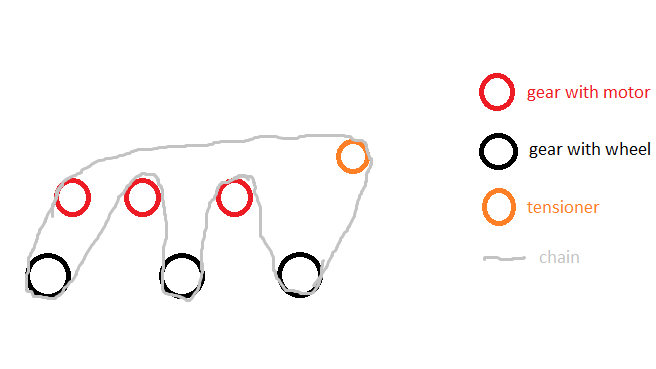
\includegraphics[scale=0.8]{days_L/Wheel_base/images/01}}
		\caption{Location of gears for chain}
	\end{minipage}
\end{figure} 



\item The first step in creating the wheelbase was making a model in Creo Parametric. Though in subsequent assembly the original design was deviated from, creating this model allowed us to establish a conceptual foundation that we were not to steer away from - usually doing so wastes time and effort.

\item To assemble the wheelbase, we needed to shorten a bar and create a chain of the exact length that was needed. In addition, the chain would slack on it's highest segment, and required careful adjustment to ensure that it would not slip while operating.

\item During tests and first competition we identified several problems:
	\begin{enumerate}
		\item Robot can't climb to ramp due to an overextension that prevented the robot from achieving the needed angle. And even if the robot was manually placed on the ramp on the needed position, it couldn't climb on top of the first churro due to low clearance. In order to fix this problem the front wheels were moved slightly forward, so that the distance between the wheel axis and the end of the beam would not exceed a certain value that is easily calculated through the angle of the ramp. After this was done, the robot could easily ride up the mountain. In order to fix the churro problem, we attached treads to the back wheels of the robot. This worked, but doing the same to all six wheels of the robot improved performance even further, and we could easily climb over the first churro in tests. However, when attempting to climb over the second churro, we found that our wheels were placed too close together:  the middle wheels pushed into the first churro and prevented the back ones from reaching the second one, and the robot would be unable to advance any further.
		
		\item Another problem we faced in first competition was the fact that our chain was not protected, and our robot could be disabled very easily just by driving into it and pulling the chain off. We added a metal sheet in front of the most exposed section of chain to protect it.
		
	\end{enumerate}
	\begin{figure}[H]
		\begin{minipage}[h]{\linewidth}
			\center{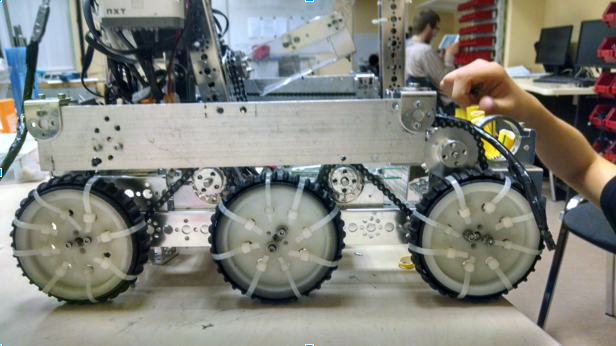
\includegraphics[scale=0.7]{days_L/Wheel_base/images/02}}
			\caption{Wheels with caterpillars and protection for chains}
		\end{minipage}
	\end{figure}
\end{itemize}
\fillpage
 

  \subsection{Lift and bucket for debris}

\subsubsection{Lift}
The lift consists of two beams. One beam is stationar and it is fixed vertically on the back part of the robot. The second beam turns by DC motor that mounted at the top of stationar beam. The length of beams must allow to score debris to high goal from the middle zone and to middle goal from low zone.	\newline
For estimating optimal length of beams it was made drawing in GeoGebra.
\begin{figure}[H]
	\begin{minipage}[h]{1\linewidth}
		\center{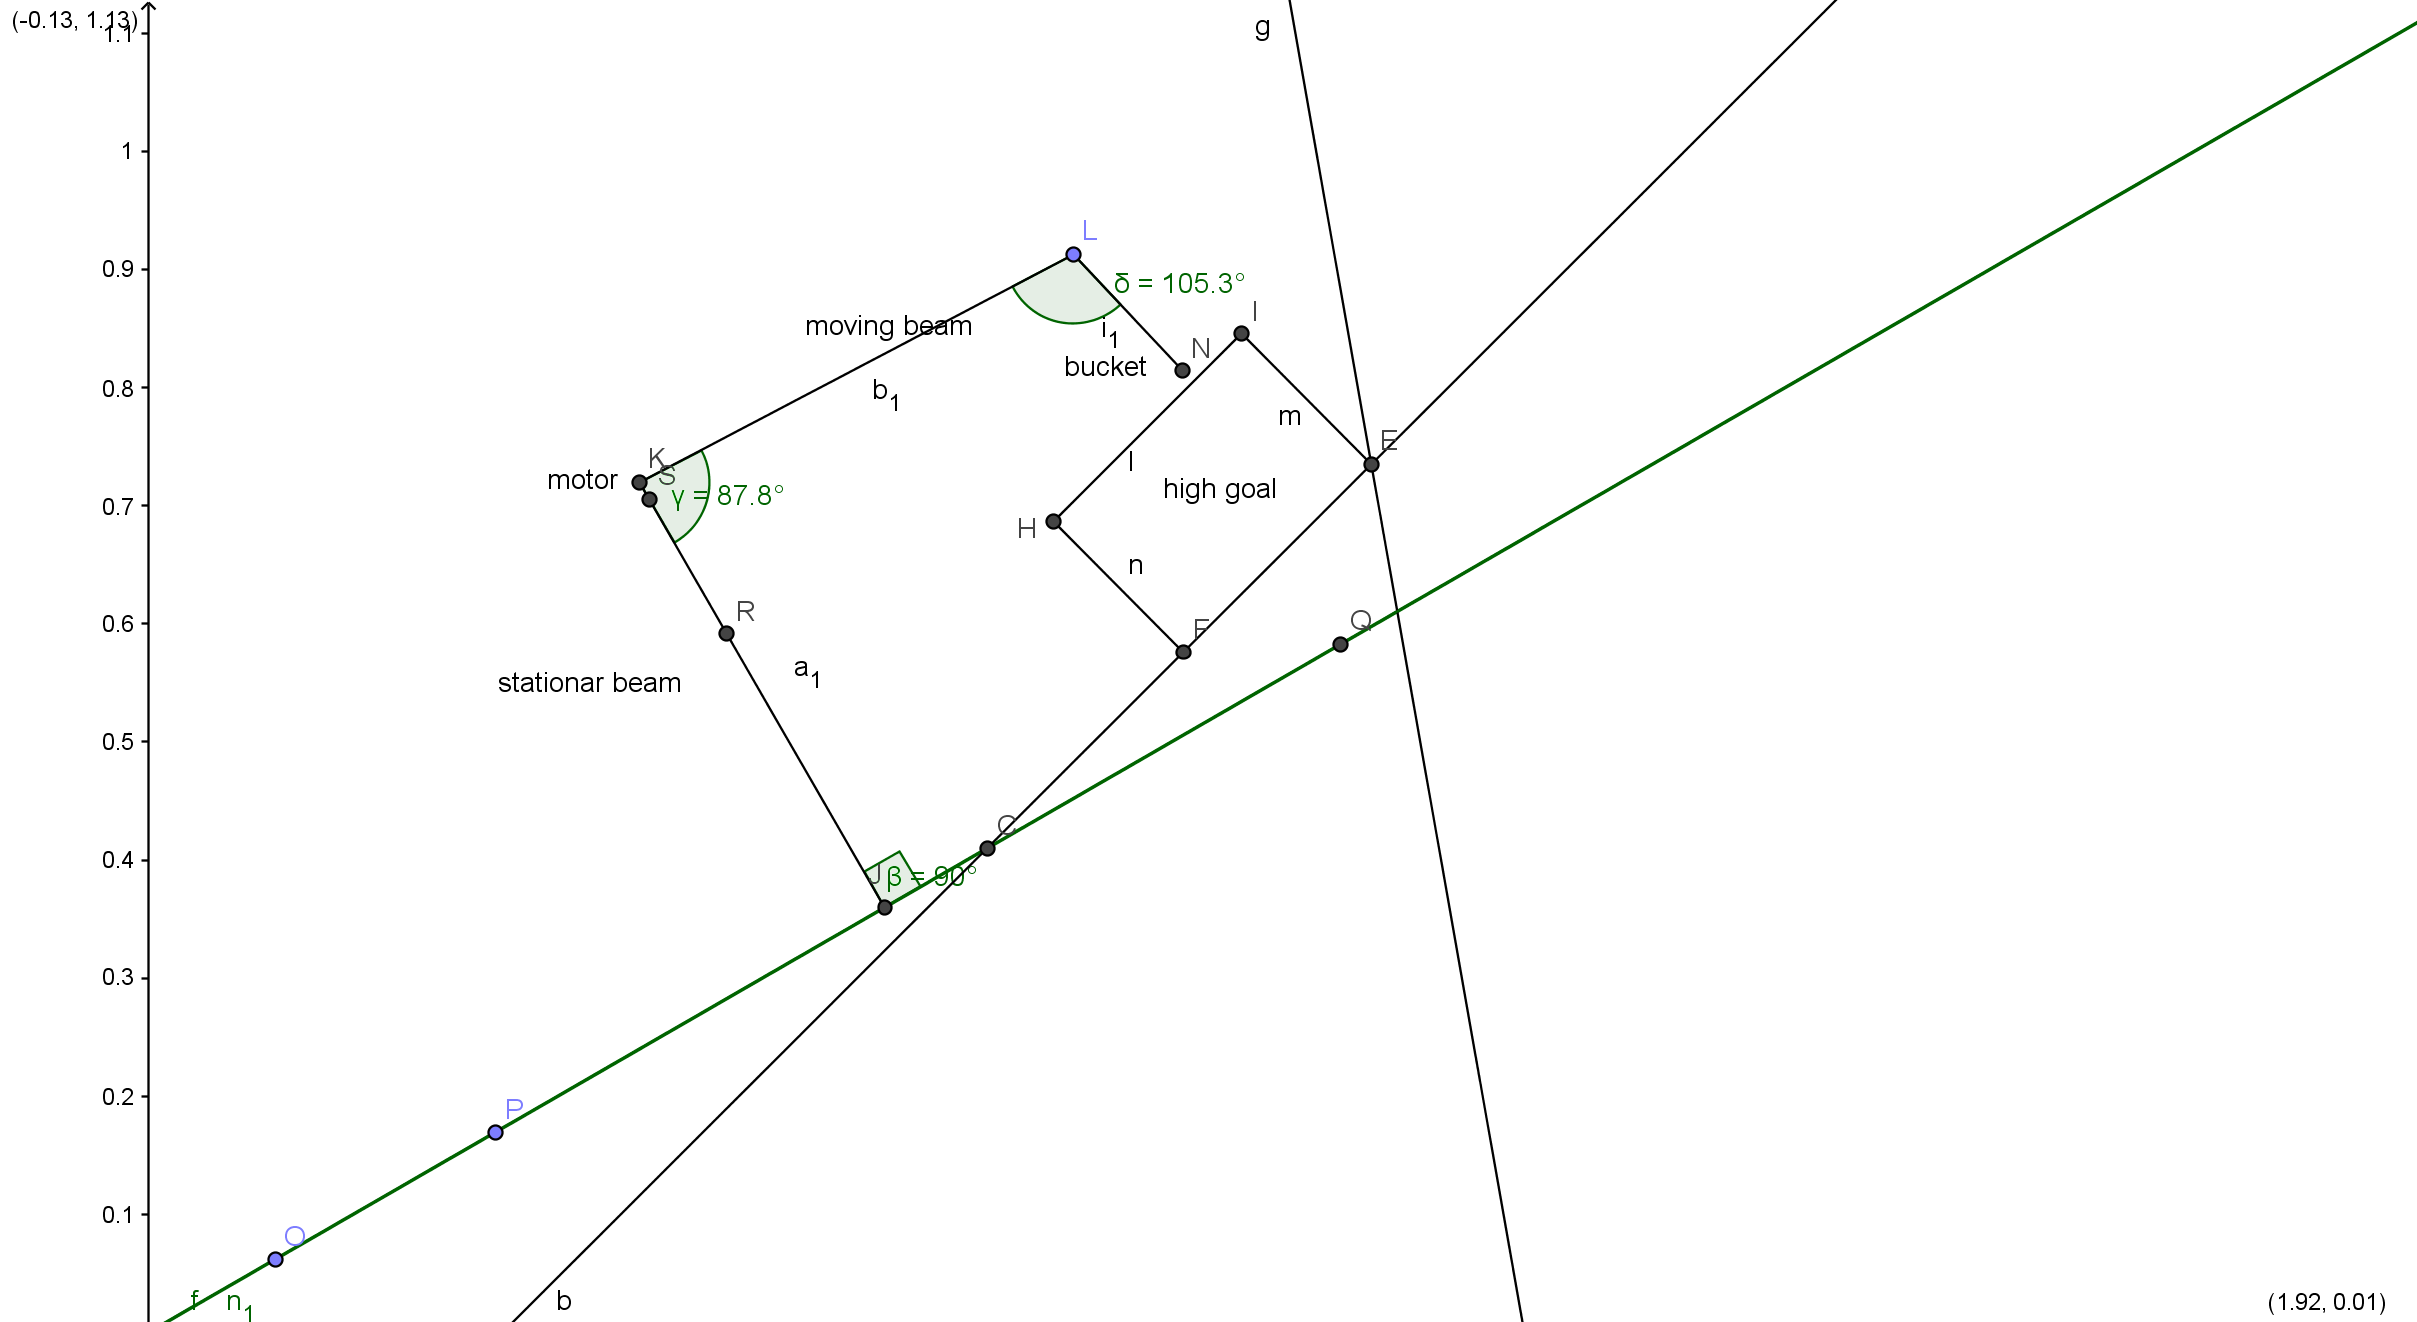
\includegraphics[scale=0.7]{days_L/Lift+bucket/images/02}}
		\caption{Drawing of the lift}
	\end{minipage}
\end{figure}

\subsubsection{Bucket} 
The bucket's size allow to fit 3 cubes and 2 balls. So we can collect 5 cubes (because size of cube is smaller than size of ball) or 3-4 balls. It is enough for us because we want to concentrate on collecting cubes. 	\newline
For estimating optimal size and form it was made drawing in GeoGebra. During designing model of the bucket for all sizes were made stocks 2cm.
\begin{figure}[H]
	\begin{minipage}[h]{1\linewidth}
		\center{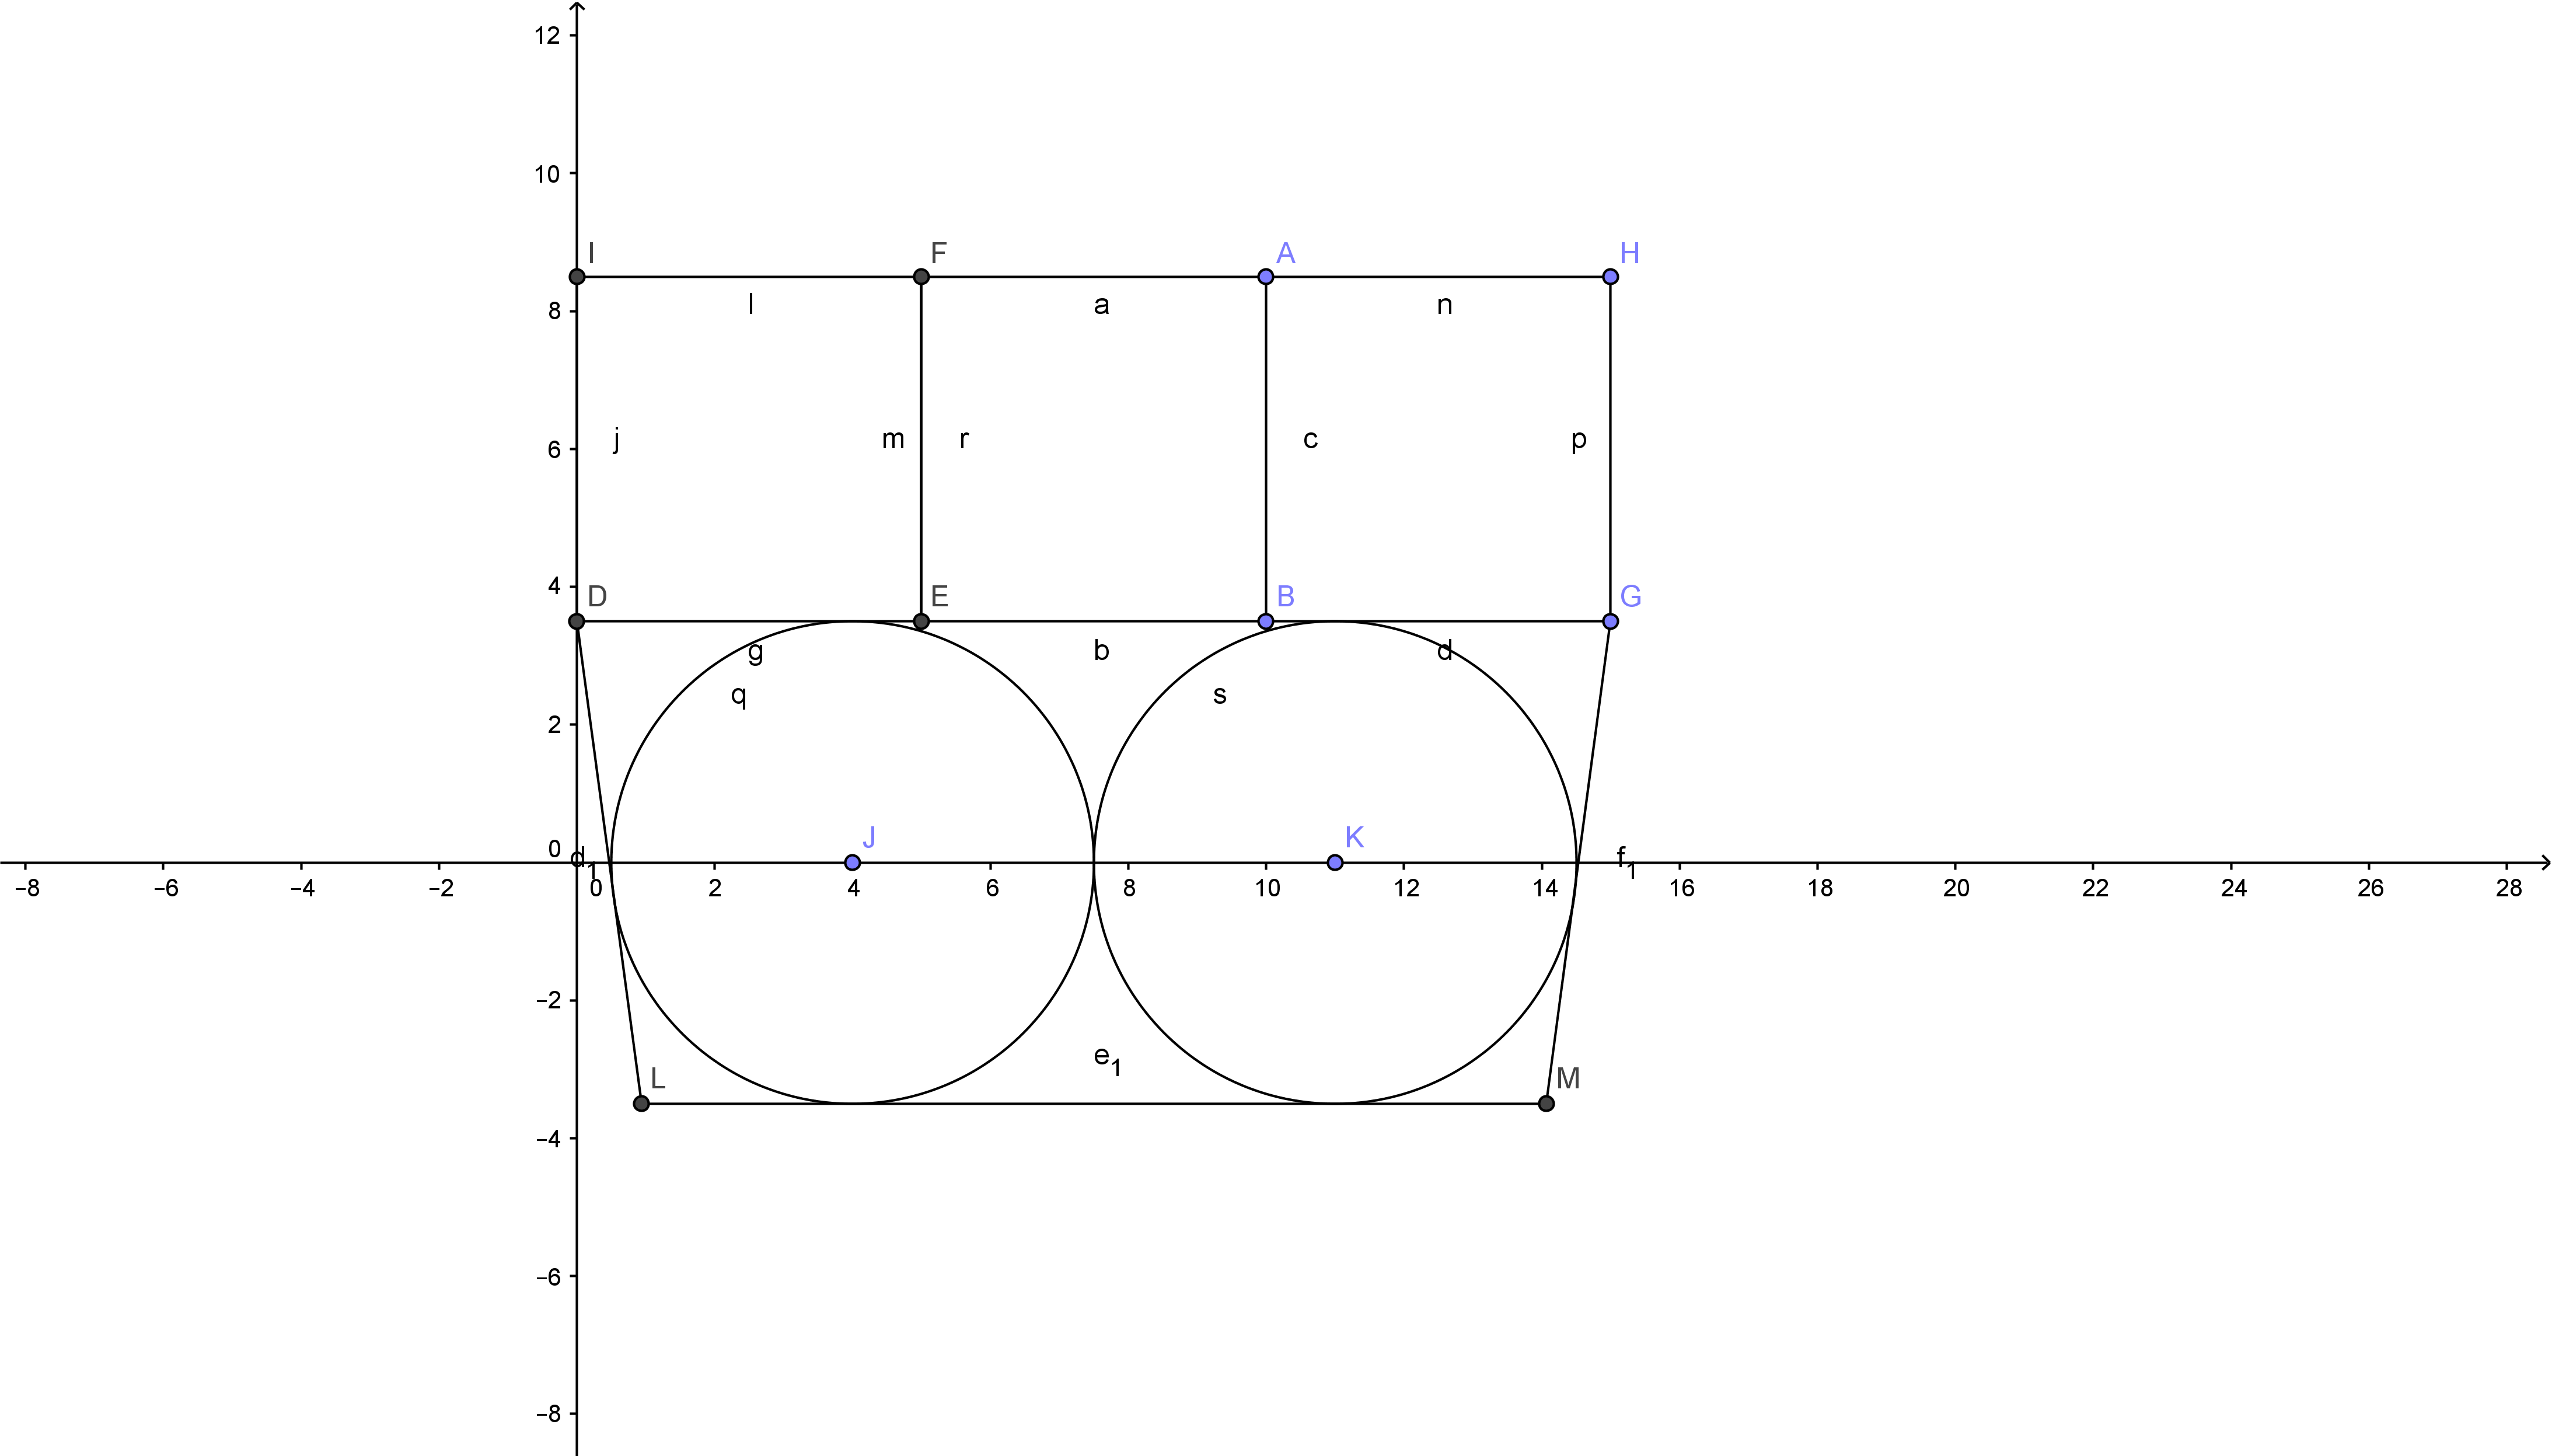
\includegraphics[scale=0.5]{days_L/Lift+bucket/images/01}}
		\caption{Drawing of the bucket}
	\end{minipage}
\end{figure}

For building bucket it was decided use plastic PET 0.5mm. It is easy to cut it, it light, cheap and clear that allow us to see how much elements are incide the bucket.\newline  

The bucket mounts to beam that turns by the servo which fixed on the lift. It need because else we have to make detail that fix bucket to the elevator on the defined angle. It require high accuracy. So it will be difficult to make this detail. In addition the mount with servo extend operational window of the lift. \newline

The bucket equped by the cover that turn by the servo and close entrance hole of the bucket. It prevent to falling debris out it during turning of the moving beam of lift. Also it can to prevent balls get into the bucket when we collect only cubes. When it closed not fully (so that distance between bottom edge of cover and floor is about 6cm) the cube can get into the bucket but the ball is not. When we open cover the balls can get to the bucket.\newline
The cover fix on 14cm beam that turn by the servo. It was decided use so long beam as the most optimal variant when cover move vertically because otherwise it can to prevent rotating gripper for debris. When it turn around the circle with big radius trajectory of cover's moving is close to vertical.


  	
   	
\fillpage

  \subsubsection{Gripper for debris}
For rotating brush it was decided use DC motor. It allow the fastest collecting debris. \newline
The first part of module is the mount to the base and axis. The brush is fixed on it.
	\begin{center}
		\begin{tabular}{|p{0.14\linewidth}|p{0.12\linewidth}|p{0.12\linewidth}|}
			{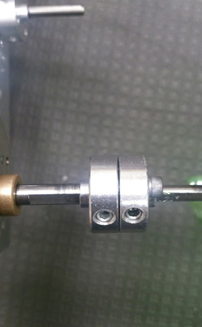
\includegraphics[scale=0.5]{days_L/Gripper/images/01}} & {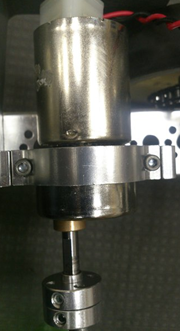
\includegraphics[scale=0.5]{days_L/Gripper/images/02}} & {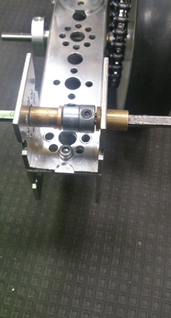
\includegraphics[scale=0.5]{days_L/Gripper/images/03}}\\
			\hline & Mount for axis  &
		\end{tabular}
	\end{center}
	Also it was made protection for wiring of the motor. It is the construction of Tetrix plates that fixed to the base rigidly.\newline
	The next element of the module is the brush. The brush should be tough enough so that it doesn't bend during collecting debris. But it should be elastic in order to when robot hit the wall of field the brush bend but not broke.\newline
	At first it was made brush made of piece of plastic bottle. During the test it collect debris good enough but it started crack.
	\begin{figure}[H]
		\begin{minipage}[h]{1\linewidth}
			\center{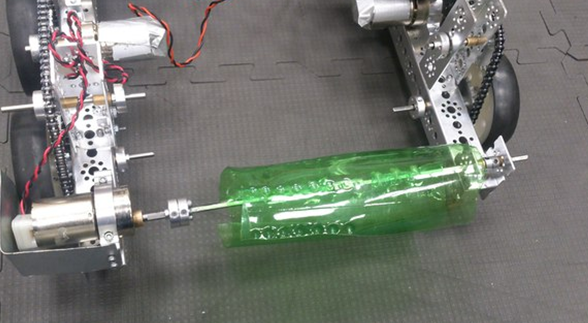
\includegraphics[scale=0.5]{days_L/Gripper/images/05}}
			\caption{Brush madde of plastic bottle}
		\end{minipage}
	\end{figure}
	So it was decided to use pieces of rubber hose because it is elastic but more durable than plastic. Pieces of hose were fixed on the aluminium tube from Tetrix set with help of screws. The tube was instaled on the shaft of motor instead of axis. This construction worked good enough. It collected debris without problems.  
	\begin{figure}[H]
		\begin{minipage}[h]{\linewidth}
			\center{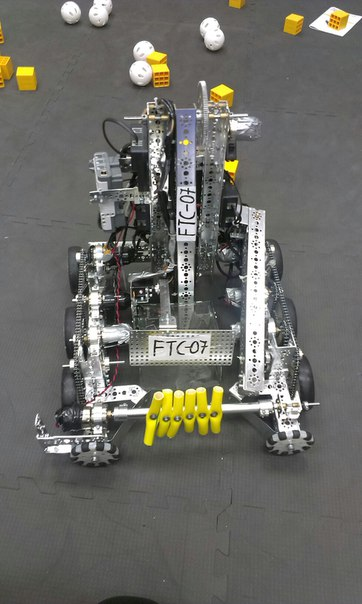
\includegraphics[scale=0.5]{days_L/Gripper/images/06}}
			\caption{Gripper with hose}
		\end{minipage}
	\end{figure}
	Later it was decided to increace speed of rotation gripper and install transmission with gear ratio 1:2. It need for pushing away scoring elements durin autonomous period.
	
\fillpage	
  \subsubsection{Mechanism for scoring autonomous climbers and pushing button}
\paragraph{Plan of creating module:}	
	
	\begin{enumerate}
		\item Creating 3D model in Creo parametric.
		\item Calculation of moments, distances and angels.
		\item Testing and debugging of the mechanism
	\end{enumerate}
	
	The module turns F-shaped beam using servo. On the top of beam is a bucket with climbers. After beam turns, bucket turns over. Climbers go to the box. At the end of other part of a beam is a light sensor. He detects color of a button and presses it. Robot performs it at autonomous period. \newline
	
	\paragraph{Ideas that were looked:}
	
	\begin{enumerate}	
		\item The first idea was the following: we decided to use two beams. Two beams turns, the light sensor on the end of each beam detects the correct button. Beam, which detects the correct button wrests in place. The other beam turns up. The robot goes forward and presses the correct button. But this idea isn't good because we using two servos and this is very difficult and the module take up much up space.
	
		\item Another idea was the following: we decided to use one beam. The beam turns and the light sensor on the end of the beam detects the color of the right button. If this color is correct, the robot turns right and then goes forward. Else the robot turns left and then goes forward. This algoritm is slower, but it's lighter and the model takes not as much space. We decided to use twice algoritm.
	\end{enumerate}
	
	\paragraph{Calculation of moments}
	
	We calculated the moments to compare it with the maximum moment of the servo. If the maximum moment of the servo is higher than the moment of module, the module will work. The maximum moment of the servo(HS-485HB) is 28 kg*mm. The moment of gravity forces using the following formulae: 
	
	$m_\text{constr} \cdot l_\text{constr} + m_\text{climbers} \cdot l_\text{climbers}$.	
	 $M_\text{constr}$ is the total mass of the module without climbers. $L_\text{constr}$ is the distance between the rotation axis and the COG of module without climber. $M_\text{climbers}$ is the total mass of the two climbers. $L_\text{climbers}$ is the distance between the rotation axis and the COG of climbers. All values we find in Creo Parametric.
	 
	 $M_\text{constr}$ is about 100 g or 0.1 kg. $L_\text{constr}$ is about 93 mm. The moment of construction is about 9.3 kg*mm. Mass of a climber is 22.7 g. Mass of two climbers is 0.0454 kg. The COG of climbers and geometrical center ar ine the same place, because the climbers are uniform. It is about 204 mm. The moment of gravity forces if the all module is 18.9 kg*mm. Safety factor is 1.5. With this factor moment of module is 28 kg*mm. The moment of module is not bigger than the maximum moment of the servo. The module will work.
	 \begin{figure}[H]
	 	\begin{minipage}[h]{\linewidth}
	 		\center{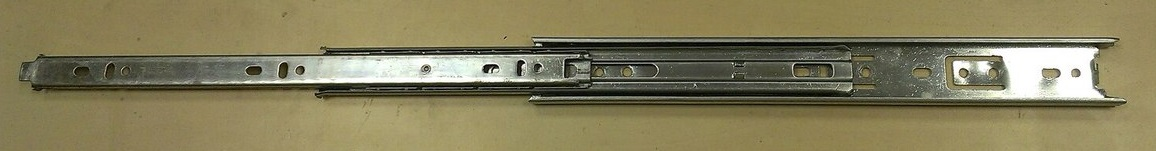
\includegraphics[scale=0.7]{days_L/f-beam/images/01}}
	 		\caption{The table of moments}
	 	\end{minipage}
	 \end{figure}
	 
	 \paragraph{Work of module}
	 
	 \begin{itemize}
	 
		 \item A dimension of the bucket is 6x5.5x12 mm. A dimenension of the main beam is 20x0.5x1.5 mm.
	 
		 \item The robot must stay near the button on the distance 16.9 cm. Also the main beam must be in the middle of the beacon. Than the robot turns beam on 48 degrees and the climbers go down. Than the robot must go forward on the distance 5 cm. After that the robot turns beam on 42 degrees. Than the robot detects correct button and turns in his side on 9 degrees. At the end the robot goes forward and presses correct button.
	\end{itemize}
	\fillpage
  
	
	%\section{Key summary}

\subsection{Model}
The final version of the model of the robot made in Creo Parametric 3.0:
\begin{figure}[H]
	\begin{minipage}[h]{1\linewidth}
		\center{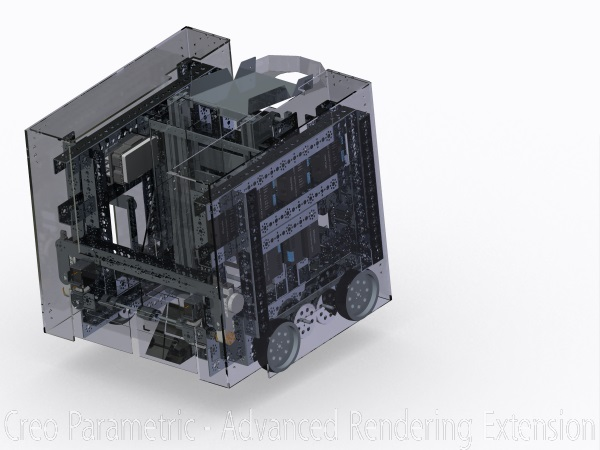
\includegraphics[scale=1]{days/Key_summary/images/A_photo}}
	\end{minipage}
\end{figure}
\begin{figure}[H]
	\begin{minipage}[h]{1\linewidth}
		\center{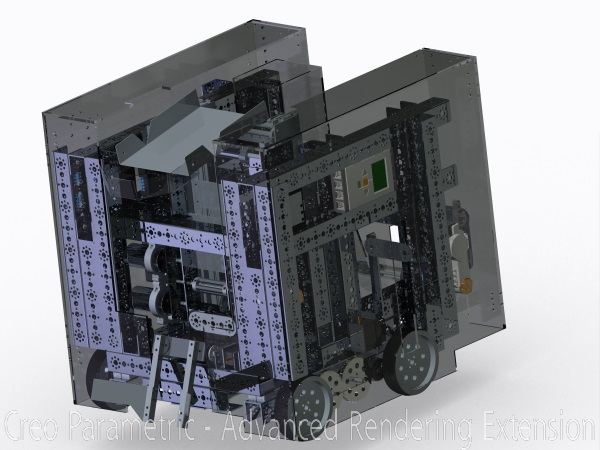
\includegraphics[scale=1]{days/Key_summary/images/A_photo2}}
	\end{minipage}
\end{figure}
\newpage
\subsection{Strategy}
Our strategy is very flexible, so we can adjust to any ally.

\newpage


	
	
\section{Thanks and prospects} 
    We enjoyed working on a custom and non-standard project, which, besides its technical aspect, included working with new people who shared our values of friendship and mutual understanding. 
    
    Our team is planning to continue doing robotics, setting new goals for ourselves in order to improve. This is our first year taking part in FTC and we will participate next year as well. If we don't realize ourselves this year, we'll look at all our mistakes, correct them, and preform a lot better next year.
   
    In any case, we are ready to learn new things, improve ourselves and expand our skills. 
    
    None of us know for sure what we want to do in the future, but we are certain that our experience will be very valuable to us. 
    
    Our thanks go to the company FIRST for organizing this competition, which we are very happy to be participating in. We appreciate this wonderful opportunity to test ourselves and learn something new and wish them success and growth in their future endeavors.
    
    Also we thank our sponsors: company PTC and it's Russian representative "Irisoft" and charitable foundation "Finist" for their support. Also we thank Physics-Mathematics Lyceum 30 and it's director Alexey Tretyakov for providing comfortable conditions for preparation to competition.
   
    
    \begin{center}
      Team PML 30 X
    \end{center}
    
    \vspace{0.5em}
    
    \begin{figure}[H]
    	\begin{minipage}[h]{0.47\linewidth}
    		\center{
\includegraphics[scale=1]{key_chapters/Thanks_for_sponsors/images/01}}
    	\end{minipage}
    	\hfill
    	\begin{minipage}[h]{0.47\linewidth}
    		\center{
\includegraphics[scale=0.2]{key_chapters/Thanks_for_sponsors/images/02}}
    	\end{minipage}
    \end{figure}
    
    \vspace{0.5em}
    
    \begin{figure}[H]
    	\begin{minipage}[h]{0.31\linewidth}
    		\center{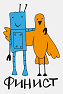
\includegraphics[scale=3]{key_chapters/Thanks_for_sponsors/images/03}}
    	\end{minipage}
    	\hfill
    	\begin{minipage}[h]{0.31\linewidth}
    		\center{
\includegraphics[scale=0.35]{key_chapters/Thanks_for_sponsors/images/05}}
    	\end{minipage}
    	\hfill
    	\begin{minipage}[h]{0.31\linewidth}
    		\center{
\includegraphics[scale=1]{key_chapters/Thanks_for_sponsors/images/04}}
    	\end{minipage}
    \end{figure}
    
    %ending:
	%\section{Appendix}



\subsection{Programm}

Program of driver control period and two versions of autonomus period with brief explanations.
\subsubsection{Driver control period}

\subsubsection{Autonomus period from the parking zone}



\subsubsection{Autonomus period from the ramp}


\subsection{Electical scheme}
The final version of the scheme of electrical components of our robot:
\begin{figure}[H]
	\begin{minipage}[h]{1\linewidth}
		\center{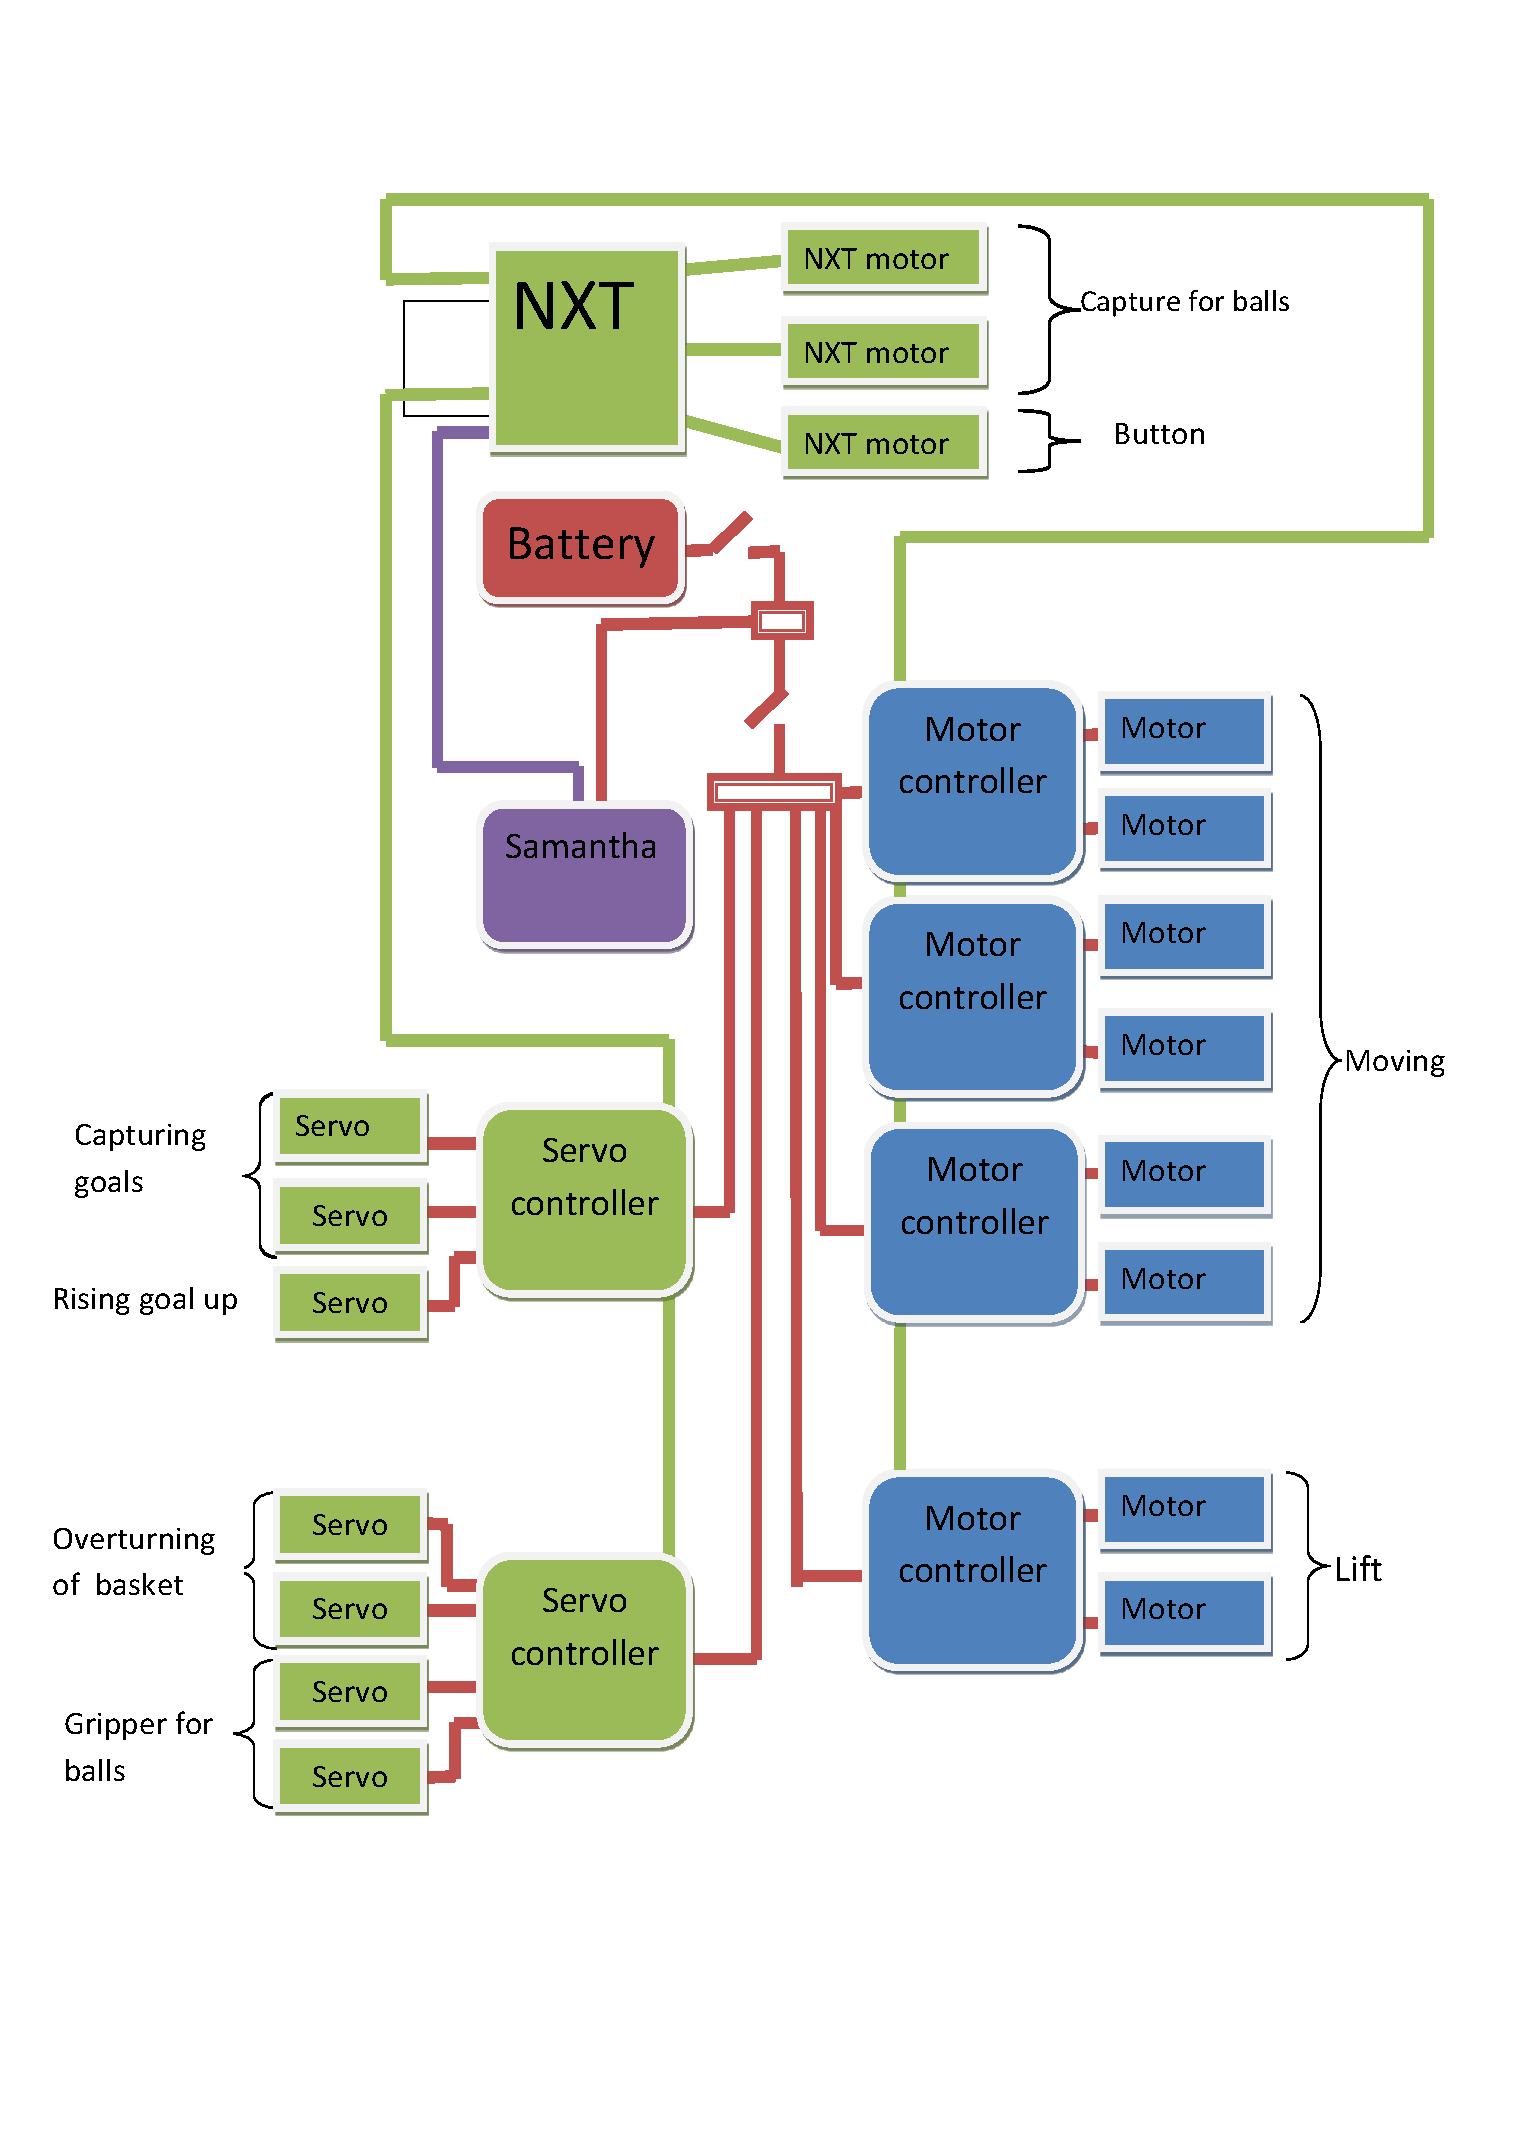
\includegraphics[scale=0.55]{days/Key_summary/images/El-scheme}}
	\end{minipage}
\end{figure}
\fillpage
	%
\subsection{Supplementary materials which were used in the robot's construction}

\begin{enumerate}
	\item Aluminium axis 1m х 8mm. 2 pieces.
	\item Steel axis 3m х 8mm. 1 piece.
	\item Aluminium strip 2m х 50mm х 2mm. 1 piece.
	\item Aluminium strip 1m х 40mm х 3mm. 1 piece.
	\item Aluminium profile 1m х 10mm х 10mm. 1 piece.
	\item Furniture slats 30сm. 2 pieces.
	\item Furniture slats 35сm. 4 pieces.
	\item Belt 2,5m. 1 piece.
	\item Plastic clamps.
	\item Plastic bottle. 1 piece.
	\item List of PET 1 m х 80 cm. 1 piece.
	\item Hot melt adhesive.
	\item Tape.
	\item List of plexiglass 3m x 2m (cut). 1 piece.
\end{enumerate}
\fillpage
\newpage



	
\end{document}
